\documentclass[twoside]{book}

% Packages required by doxygen
\usepackage{fixltx2e}
\usepackage{calc}
\usepackage{doxygen}
\usepackage[export]{adjustbox} % also loads graphicx
\usepackage{graphicx}
\usepackage[utf8]{inputenc}
\usepackage{makeidx}
\usepackage{multicol}
\usepackage{multirow}
\PassOptionsToPackage{warn}{textcomp}
\usepackage{textcomp}
\usepackage[nointegrals]{wasysym}
\usepackage[table]{xcolor}

% Font selection
\usepackage[T1]{fontenc}
\usepackage[scaled=.90]{helvet}
\usepackage{courier}
\usepackage{amssymb}
\usepackage{sectsty}
\renewcommand{\familydefault}{\sfdefault}
\allsectionsfont{%
  \fontseries{bc}\selectfont%
  \color{darkgray}%
}
\renewcommand{\DoxyLabelFont}{%
  \fontseries{bc}\selectfont%
  \color{darkgray}%
}
\newcommand{\+}{\discretionary{\mbox{\scriptsize$\hookleftarrow$}}{}{}}

% Page & text layout
\usepackage{geometry}
\geometry{%
  a4paper,%
  top=2.5cm,%
  bottom=2.5cm,%
  left=2.5cm,%
  right=2.5cm%
}
\tolerance=750
\hfuzz=15pt
\hbadness=750
\setlength{\emergencystretch}{15pt}
\setlength{\parindent}{0cm}
\setlength{\parskip}{3ex plus 2ex minus 2ex}
\makeatletter
\renewcommand{\paragraph}{%
  \@startsection{paragraph}{4}{0ex}{-1.0ex}{1.0ex}{%
    \normalfont\normalsize\bfseries\SS@parafont%
  }%
}
\renewcommand{\subparagraph}{%
  \@startsection{subparagraph}{5}{0ex}{-1.0ex}{1.0ex}{%
    \normalfont\normalsize\bfseries\SS@subparafont%
  }%
}
\makeatother

% Headers & footers
\usepackage{fancyhdr}
\pagestyle{fancyplain}
\fancyhead[LE]{\fancyplain{}{\bfseries\thepage}}
\fancyhead[CE]{\fancyplain{}{}}
\fancyhead[RE]{\fancyplain{}{\bfseries\leftmark}}
\fancyhead[LO]{\fancyplain{}{\bfseries\rightmark}}
\fancyhead[CO]{\fancyplain{}{}}
\fancyhead[RO]{\fancyplain{}{\bfseries\thepage}}
\fancyfoot[LE]{\fancyplain{}{}}
\fancyfoot[CE]{\fancyplain{}{}}
\fancyfoot[RE]{\fancyplain{}{\bfseries\scriptsize Generated by Doxygen }}
\fancyfoot[LO]{\fancyplain{}{\bfseries\scriptsize Generated by Doxygen }}
\fancyfoot[CO]{\fancyplain{}{}}
\fancyfoot[RO]{\fancyplain{}{}}
\renewcommand{\footrulewidth}{0.4pt}
\renewcommand{\chaptermark}[1]{%
  \markboth{#1}{}%
}
\renewcommand{\sectionmark}[1]{%
  \markright{\thesection\ #1}%
}

% Indices & bibliography
\usepackage{natbib}
\usepackage[titles]{tocloft}
\setcounter{tocdepth}{3}
\setcounter{secnumdepth}{5}
\makeindex

% Hyperlinks (required, but should be loaded last)
\usepackage{ifpdf}
\ifpdf
  \usepackage[pdftex,pagebackref=true]{hyperref}
\else
  \usepackage[ps2pdf,pagebackref=true]{hyperref}
\fi
\hypersetup{%
  colorlinks=true,%
  linkcolor=blue,%
  citecolor=blue,%
  unicode%
}

% Custom commands
\newcommand{\clearemptydoublepage}{%
  \newpage{\pagestyle{empty}\cleardoublepage}%
}

\usepackage{caption}
\captionsetup{labelsep=space,justification=centering,font={bf},singlelinecheck=off,skip=4pt,position=top}

%===== C O N T E N T S =====

\begin{document}

% Titlepage & ToC
\hypersetup{pageanchor=false,
             bookmarksnumbered=true,
             pdfencoding=unicode
            }
\pagenumbering{alph}
\begin{titlepage}
\vspace*{7cm}
\begin{center}%
{\Large ci\+\_\+example\+\_\+python }\\
\vspace*{1cm}
{\large Generated by Doxygen 1.8.13}\\
\end{center}
\end{titlepage}
\clearemptydoublepage
\pagenumbering{roman}
\tableofcontents
\clearemptydoublepage
\pagenumbering{arabic}
\hypersetup{pageanchor=true}

%--- Begin generated contents ---
\chapter{ci\+\_\+example\+\_\+python}
\label{index}\hypertarget{index}{}\subsection*{What is it}

This package contains a set of examples of demos and unit tests in c++ supported by the continuous integration. It also contains the coding guidelines setup in the \href{https://wp.nyu.edu/machinesinmotion/}{\tt machines-\/in-\/motion} group.

\subsection*{Authors}


\begin{DoxyItemize}
\item Vincent Berenz
\item Maximilien Naveau
\end{DoxyItemize}

\subsection*{Copyrights}

Copyright (c) 2019, New York University and Max Planck Gesellschaft.

\subsection*{License}

License B\+S\+D-\/3-\/\+Clause 
\chapter{List of flake8 Plugins for Popular Editors}
\label{md_doc_flake8_plugins}
\Hypertarget{md_doc_flake8_plugins}
Feel free to extend the list if you find a plugin for an editor not yet listed here or a better plugin for one that is already listed.

Note that you need to be careful to use flake8 for the correct Python version.

\subsection*{Visual Studio Code}

VS Code already has built-\/in support for flake8 but it needs to be enabled in the configuration. See \href{https://code.visualstudio.com/docs/python/linting}{\tt the official documentation} for instructions.

\subsection*{Vim}

\subsubsection*{Syntastic}

\href{https://github.com/vim-syntastic/syntastic}{\tt Syntastic} is a plugin for running external style checkers that can run flake8. \begin{DoxyVerb}let g:syntastic_python_checkers = ['flake8']
" to ensure flake8 checks for python 3 code:
let g:syntastic_python_flake8_exe = 'python3 -m flake8'
\end{DoxyVerb}


\subsubsection*{A\+LE}

\href{https://github.com/dense-analysis/ale}{\tt A\+LE} is a plugin for running linters asynchronously. As it runs the linter in the background, it is preferable over Syntastic, however, it needs Vim version 8 or later or Neovim.

To ensure using flake for Python 3, use the following configuration\+: \begin{DoxyVerb}let g:ale_python_flake8_executable = 'python3'
let g:ale_python_flake8_options = '-m flake8'\end{DoxyVerb}
 
\chapter{1. General rules applied in the code base}
\label{coding_guidelines_0}
\Hypertarget{coding_guidelines_0}
\subsection*{I. Introduction}

These are general rules independent of the coding language.

\subsection*{II. Catkin Package and Repository Naming}


\begin{DoxyItemize}
\item Name\+: lower\+\_\+cases\+\_\+with\+\_\+underscore.
\item One repository per catkin package.
\item Same name for package and repository.
\end{DoxyItemize}

\subsection*{I\+II. Versioning}

Use semantic versioning when versioning packages. Short summary\+:


\begin{DoxyItemize}
\item Given a version number M\+A\+J\+O\+R.\+M\+I\+N\+O\+R.\+P\+A\+T\+CH, increment the\+:
\item M\+A\+J\+OR version when you make incompatible A\+PI changes,
\item M\+I\+N\+OR version when you add functionality in a backwards-\/compatible manner, and
\item P\+A\+T\+CH version when you make backwards-\/compatible bug fixes.
\end{DoxyItemize}

Regarding formatting of pre-\/releases (alpha, beta, rc, ...) consider P\+E\+P440, especially when versioning Python packages (note that there is no general conflict with semantic versioning, only the format is a bit different).

\subsection*{IV. Contribution Guidelines}

\subsubsection*{I\+V.\+1. Code revision\+:}

To ensure some level of code quality, all modifications have to be reviewed before they can be merged. This is done via merge requests in Git\+Lab (on Git\+Hub it is called pull request but the concept is the same).

The procedure for adding a change is as follows\+:


\begin{DoxyItemize}
\item When creating branches, use your name as a namespace, e.\+g. {\itshape rickdeckard/my\+\_\+branch}. This is to avoid confusion with branches of other people and to indicate who is responsible for that branch. It is not allowed to push branches without such namespace.
\item Test all your changes and update documentation.
\item When finished, create a merge request to the master branch of the main repository.
\item Add one or more of the maintainers as reviewers. The reviewers will review and maybe request changes.
\item Merging is done by the contributor but is only allowed after all reviewers approved. If the merge will affect other people (e.\+g. by breaking the A\+PI), make sure to inform them, e.\+g. via a Mail on an appropriate mailing list. After a merge request is merged, the feature branch shall be deleted.
\end{DoxyItemize}

Never push directly to master or other top-\/level branches. Never force-\/push to any branch that others are using as well. All your development should happen in branches inside your namespace. To keep the number of branches on the repository low, make sure to delete branches that are not needed anymore.

The top-\/level namespace of the repository should only contain a master branch and maybe a few branches for specific versions. Those branches should be protected so that direct pushing is not possible (everything has to go through merge requests).

\subsubsection*{I\+V.\+2. Some rules for the contributors\+:}


\begin{DoxyItemize}
\item To make life easier for the reviewers and to get your changes merged quickly (thus reducing the risk of merge conflicts), try to keep merge requests rather small. This means that, where possible, a bigger task should be split into smaller sub-\/tasks that can be merged one after another instead of putting everything in one huge merge request.
\item When synchronising your feature branch with upstream, you may want to prefer git rebase over git merge to keep the history of you branch clean. However, when there are complicated merge conflicts, it can be much less painful to use merge, which is okay in this case.
\item On your own branches, you can do whatever you want, i.\+e. it is usually okay to force push there (and even necessary when you rebase). However, when applying changes requested by a reviewer, please do not amend or squash them into older commits but add them as new commits. This makes it easier for the reviewer to see what changed.
\item Do not add functional changes and major reformatting in the same commit as this makes review of the functional changes very difficult.
\item Do add unit tests for new features
\item Do create new demos or update existing demos to make it easier how to use the updated A\+PI
\end{DoxyItemize}

\subsubsection*{I\+V.\+3. Some rules for the reviewers\+:}


\begin{DoxyItemize}
\item To make life easier for the contributors, try to provide reviews in a timely manner. The contributor may be blocked in continuing their work while the merge request is under review.
\item When reviewing, check the following things\+:
\begin{DoxyItemize}
\item Is the style guide followed?
\item Are new features/changes properly documented?
\item And of course\+: Do the changes look reasonable and correct?
\end{DoxyItemize}
\item The one who merges should directly delete the feature branch afterwards.
\end{DoxyItemize}

\subsection*{V. Documentation}

\subsubsection*{V.\+1 In-\/code documentation}

All code {\bfseries shall} be documented in-\/source using Doxygen. This means that every function, class, struct, global variable, etc, needs to have a docstring containing some documentation in\+:
\begin{DoxyItemize}
\item \href{https://google.github.io/styleguide/pyguide.html?showone=Comments#Comments}{\tt Google} format for Python,
\item \href{http://www.doxygen.nl/manual/index.html}{\tt Doxygen} format for C/\+C++.
\end{DoxyItemize}

If the definition and declaration are separated (C/\+C++), Doxygen should be in the header, not the cpp file. {\bfseries Please do not duplicate!}.

If you are using catkin, the package should include the mpi\+\_\+cmake\+\_\+modules package and in the C\+Make\+Lists.\+txt file call the {\ttfamily build\+\_\+doxygen\+\_\+documentation()} or the {\ttfamily default\+\_\+mpi\+\_\+cmake\+\_\+modules()}(future) macros. The documentation can then be build via catkin\+\_\+make -\/\+D\+B\+U\+I\+L\+D\+\_\+\+D\+O\+C\+U\+M\+E\+N\+T\+A\+T\+I\+ON=ON.

Make the documentation as compact as possible. Avoid boilerplate formulations that do not add useful information, e.\+g. instead of \char`\"{}\+This function returns foobar\char`\"{} simply write \char`\"{}\+Returns foobar\char`\"{}.

Also add regular comments to the code whenever you feel that they would help a future reader to more easily understand what that code is doing.

\subsubsection*{V.\+2 Unit-\/tests and demos}

Please do {\bfseries N\+OT} neglect the power of the continuous intergation and a nice written demos in terms of Documentation. So {\bfseries please} take the time to\+:
\begin{DoxyItemize}
\item write some unit-\/tests. See how to write a unit-\/tests from the tests folder in this package.
\item write demo executables to make the external user understand how your A\+PI should be used. 
\end{DoxyItemize}
\chapter{2. Python Coding Guidelines}
\label{coding_guidelines_1}
\Hypertarget{coding_guidelines_1}
\subsection*{I. Introduction}

These are the internal C++ guidelines for the \href{https://wp.nyu.edu/machinesinmotion/}{\tt machines-\/in-\/motion} group. The same guidelines are used in the \href{https://open-dynamic-robot-initiative.github.io/}{\tt Open Dynamic Robot Initiative}

The following rules present basic guidelines for our C++ code. The goal is to have code that is formatted in a consistent and easily readable way while at the same time not being overly complicated by specifying every detail. For such guidelines to be practical, newcomers should be able to read them within a few minutes and be able to memorize them. So these rules intentionally do not cover every detail but rather aim at specifying only the big, important things.

If this is too simple for you and you want more rules, you are encouraged to read the \href{https://google.github.io/styleguide/cppguide.html}{\tt Google C++ Style Guide} on which these rules are based. Note, however, that we have a few small deviations from the Google style.

These guidelines may evolve in time so it is first good practice to check them upon creation of a new package or code refactoring.

\subsection*{II. Folder Structure and File Naming}


\begin{DoxyItemize}
\item Header files should be in a folder\+: {\ttfamily include/$<$name\+\_\+of\+\_\+the\+\_\+project$>$/$\ast$}, e.\+g.
\begin{DoxyCode}
`#include "ci\_example\_cpp/gains\_configuration.hpp"` 
\end{DoxyCode}

\item File extension for header files\+: {\ttfamily .hpp}
\item Source files should be in a folder named {\ttfamily src/}. The file should have the same name as the header with extension {\ttfamily .cpp}.
\item When using templates\+: If you want to separate declaration and definition, put the declaration to a {\ttfamily .hpp} header file as usual and the definition to a file with extension {\ttfamily .hxx} in the same directory (which is included at the bottom of the {\ttfamily .hpp} file).
\item Preferably each class should be in a separate file with name {\itshape class\+\_\+name\+\_\+in\+\_\+lower\+\_\+case}. However, this is not a strict rule, if several smaller classes are logically closely related, they may go to the same file.
\item Executable scripts should be placed in the {\ttfamily scripts/} folder. And should have a C\+Make {\bfseries install rule} that makes them executable upon installation.
\item The C++/pybind11 code for wrapping C++ code to Python must be placed in {\ttfamily srcpy/}
\end{DoxyItemize}

\subsection*{I\+II. Naming}

Give as descriptive a name as possible, within reason. Do not worry about saving horizontal space as it is far more important to make your code immediately understandable by a new reader. Do not use abbreviations that are ambiguous or unfamiliar to readers outside your project, and do not abbreviate by deleting letters within a word. Abbreviations that would be familiar to someone outside your project with relevant domain knowledge are OK. As a rule of thumb, an abbreviation is probably OK if it\textquotesingle{}s listed in Wikipedia.

Formatting of names should be as follows\+:


\begin{DoxyItemize}
\item types (classes, structs, ...)\+: {\itshape First\+Upper\+Camel\+Case}
\item functions, methods\+: {\itshape lower\+\_\+case\+\_\+with\+\_\+underscores}
\item variables\+: {\itshape lower\+\_\+case\+\_\+with\+\_\+underscores}
\item class members\+: {\itshape like\+\_\+variables\+\_\+but\+\_\+with\+\_\+trailing\+\_\+underscore\+\_\+}
\item constants\+: {\itshape U\+P\+P\+E\+R\+\_\+\+C\+A\+S\+E\+\_\+\+W\+I\+T\+H\+\_\+\+U\+N\+D\+E\+R\+S\+C\+O\+R\+ES}
\item global variables\+: Should generally be avoided but if needed, prefix them with g\+\_\+, i.\+e. {\itshape g\+\_\+variable\+\_\+name}.
\end{DoxyItemize}

\subsection*{IV. Add Units to Variable Names}

Variables that hold values of a specific unit should have that unit appended to the name. For example if a variable holds the velocity of a motor in {\itshape krpm} it should be called {\ttfamily velocity\+\_\+krpm} instead of {\ttfamily just velocity}. Some more examples\+:


\begin{DoxyItemize}
\item duration\+\_\+us (use \char`\"{}u\char`\"{} instead of \char`\"{}µ\char`\"{})
\item voltage\+\_\+mV
\item acceleration\+\_\+mps2 ( $ \frac{m}{s^2} $)
\end{DoxyItemize}

\subsection*{V. C/\+C++ Formatting}

\subsubsection*{V.\+1. Line Length}

Limit the length of lines to 80 characters.

This may seem hard to follow sometimes but makes it much easier to view two or even three files next to each other (important during code review or when resolving merge conflicts).

\subsubsection*{V.\+2. Indentation}


\begin{DoxyItemize}
\item Use spaces instead of tabs.
\item 4 spaces per \char`\"{}tab\char`\"{}.
\end{DoxyItemize}

\subsubsection*{V.\+3. Position of braces}


\begin{DoxyItemize}
\item Opening brace always goes to the next line.
\item {\bfseries Always} add braces for single-\/line if/loop/etc.
\end{DoxyItemize}

Example\+:


\begin{DoxyCode}
\textcolor{keyword}{namespace }bar
\{

\textcolor{keyword}{class }Foo
\{
    \textcolor{keywordtype}{void} my\_function(\textcolor{keyword}{const} Foo &foo, \textcolor{keywordtype}{int} *output\_arg)
    \{
        \textcolor{keywordflow}{if} (condition)
        \{
            ...
        \}
        \textcolor{keywordflow}{else} \textcolor{keywordflow}{if} (other\_condition)
        \{
            ...
        \}
        \textcolor{keywordflow}{else}
        \{
            ...
        \}

        \textcolor{keywordflow}{while} (condition)
        \{
            ...
        \}
    \}
\}

\} \textcolor{comment}{// namespace}
\end{DoxyCode}


\subsubsection*{V.\+3. Spaces}

Add single spaces between if/for/etc., the condition and the brace. add spaces around most binary operators. Exception\+: No spaces around {\ttfamily \+:\+:}, {\ttfamily .} and {\ttfamily -\/$>$}. Also no spaces for unary operators ({\ttfamily i++}, {\ttfamily \&x}, {\ttfamily $\ast$x}, ...).

Example\+: 
\begin{DoxyCode}
\textcolor{keywordtype}{int} x = 42;
\textcolor{keywordflow}{for} (\textcolor{keywordtype}{int} i = 0; i < x; i++)
\{
    \textcolor{keywordtype}{int} y = i * x;
    \textcolor{keywordflow}{if} (y == foo.bar->baz)
    \{
        ...
    \}
\}
\end{DoxyCode}


\subsubsection*{V.\+4. Formatting of switch blocks}


\begin{DoxyItemize}
\item See the following example for proper indentation of switch blocks.
\item Always add a default case, even when it is technically not needed.
\begin{DoxyItemize}
\item If the default block is empty, it shall contain a comment to indicate that this is intentional.
\item The default case shall either be the first or the last case, preferably the last.
\end{DoxyItemize}
\item Non-\/empty cases shall be terminated by an unconditional break.
\end{DoxyItemize}


\begin{DoxyCode}
\textcolor{keywordflow}{switch} (x)
\{
    \textcolor{keywordflow}{case} 1:
        \textcolor{comment}{// ...}
        \textcolor{keywordflow}{break};

    \textcolor{keywordflow}{case} 2:
        \textcolor{comment}{// ...}
        \textcolor{keywordflow}{break};

    \textcolor{keywordflow}{case} 3: \textcolor{comment}{// multiple cases for one block are okay}
    \textcolor{keywordflow}{case} 4:
        \textcolor{comment}{// ...}
        \textcolor{keywordflow}{break};

    \textcolor{keywordflow}{case} 5:           \textcolor{comment}{// BAD. A non-empty case without break should not be}
        something();  \textcolor{comment}{// used}
    \textcolor{keywordflow}{case} 6:
        more();
        \textcolor{keywordflow}{break};

    \textcolor{keywordflow}{default}:
        \textcolor{comment}{// no action needed}
        \textcolor{keywordflow}{break};
\}
\end{DoxyCode}


\subsubsection*{V.\+5. Clang-\/\+Format Configuration}

To automatically format your code according to this guidelines, you can use clang-\/format with the configuration \href{https://github.com/machines-in-motion/mpi_cmake_modules/blob/master/python/mpi_cmake_modules/_clang-format}{\tt here}.

\subsection*{VI. C/\+C++ Coding Guidelines}

\subsubsection*{V\+I.\+1. Pass objects by const reference}

In general, non-\/primitive data types should be passed to functions by const reference instead of by value.


\begin{DoxyCode}
\textcolor{keywordtype}{void} foobar(\textcolor{keyword}{const} Foo &foo);  \textcolor{comment}{// good}
\textcolor{keywordtype}{void} foobar(Foo foo);  \textcolor{comment}{// results in copy of `foo`. Only do this if const}
                       \textcolor{comment}{// reference is not possible for some reason.}
\end{DoxyCode}


\#\#\# V\+I.\+2.
\begin{DoxyCode}
*#pragma once* 
\end{DoxyCode}
 vs Include Guards

Prefer
\begin{DoxyCode}
*#pragma once* 
\end{DoxyCode}
 over include guards. 
\begin{DoxyCode}
*#pragma once* 
\end{DoxyCode}
 is not part of the official standard but is widely supported by compilers and much simpler to maintain.

Note that there are some border cases where
\begin{DoxyCode}
*#pragma once* 
\end{DoxyCode}
 is causing issues (e.\+g. on Windows or when having a weird build setup with symlinks or copies of files). In such cases use traditional include guards. Make sure they have unique names by composing them from the package name and the path/name of the file (e.\+g. M\+Y\+\_\+\+P\+A\+C\+K\+A\+G\+E\+\_\+\+P\+A\+T\+H\+\_\+\+T\+O\+\_\+\+F\+I\+L\+E\+\_\+\+F\+I\+L\+E\+N\+A\+M\+E\+\_\+H). Please {\bfseries do not} add underscore as prefix nor suffix beccause this is reserved for the compiler preproccesor variables.

\subsubsection*{V\+I.\+3. Keep scopes small}

Avoid adding anything to the global namespace if possible. This means


\begin{DoxyItemize}
\item Use a namespace when defining extern symbols.
\item Use an anonymous namespace or static for symbols that are only used internally.
\end{DoxyItemize}

Generally define symbols in the smallest possible scope, i.\+e. if a variable is only used inside one loop, define it inside this loop (however, do not consider this to be a very strict rule, deviate from it where it seems reasonable).

\subsubsection*{V\+I.\+4. Use types with explicit sizes}

The header stdint defines primitive types with explicit sizes\+: {\itshape int32\+\_\+t}, {\itshape uint32\+\_\+t}, {\itshape int16\+\_\+t}, ... They should be preferred over the build-\/in types int, unsigned, short, ... To use them add the following include\+: 
\begin{DoxyCode}
\textcolor{preprocessor}{#include <stdint>}
\end{DoxyCode}
 
\chapter{Namespace Index}
\section{Namespace List}
Here is a list of all documented namespaces with brief descriptions\+:\begin{DoxyCompactList}
\item\contentsline{section}{\hyperlink{namespacedynamic__graph}{dynamic\+\_\+graph} \\*This is this package namespace in order to avoid naming conflict }{\pageref{namespacedynamic__graph}}{}
\item\contentsline{section}{\hyperlink{namespacedynamic__graph_1_1specific}{dynamic\+\_\+graph\+::specific} \\*Types dedicated to identify pairs of (dg,ros) data }{\pageref{namespacedynamic__graph_1_1specific}}{}
\item\contentsline{section}{\hyperlink{namespacedynamic__graph__manager}{dynamic\+\_\+graph\+\_\+manager} \\*Example of hardware communication client based on R\+OS }{\pageref{namespacedynamic__graph__manager}}{}
\item\contentsline{section}{\hyperlink{namespacedynamicgraph}{dynamicgraph} \\*Definition of the command }{\pageref{namespacedynamicgraph}}{}
\item\contentsline{section}{\hyperlink{namespacedynamicgraph_1_1command}{dynamicgraph\+::command} \\*This is this the namespace including the commands }{\pageref{namespacedynamicgraph_1_1command}}{}
\item\contentsline{section}{\hyperlink{namespacedynamicgraph_1_1command_1_1ros__state__publish}{dynamicgraph\+::command\+::ros\+\_\+state\+\_\+publish} \\*This is this a namespace including the ros state publisher command }{\pageref{namespacedynamicgraph_1_1command_1_1ros__state__publish}}{}
\end{DoxyCompactList}

\chapter{Hierarchical Index}
\section{Class Hierarchy}
This inheritance list is sorted roughly, but not completely, alphabetically\+:\begin{DoxyCompactList}
\item array\+\_\+members\begin{DoxyCompactList}
\item \contentsline{section}{shared\+\_\+memory\+:\+:array$<$ T, S\+I\+ZE $>$}{\pageref{classshared__memory_1_1array}}{}
\end{DoxyCompactList}
\item \contentsline{section}{shared\+\_\+memory\+:\+:Condition\+Variable}{\pageref{classshared__memory_1_1ConditionVariable}}{}
\item \contentsline{section}{Config}{\pageref{classConfig}}{}
\item exception\begin{DoxyCompactList}
\item \contentsline{section}{shared\+\_\+memory\+:\+:Allocation\+\_\+exception}{\pageref{classshared__memory_1_1Allocation__exception}}{}
\item \contentsline{section}{shared\+\_\+memory\+:\+:Memory\+\_\+overflow\+\_\+exception}{\pageref{classshared__memory_1_1Memory__overflow__exception}}{}
\item \contentsline{section}{shared\+\_\+memory\+:\+:Not\+\_\+consumed\+\_\+exception}{\pageref{classshared__memory_1_1Not__consumed__exception}}{}
\item \contentsline{section}{shared\+\_\+memory\+:\+:Unexpected\+\_\+map\+\_\+key$<$ Key $>$}{\pageref{classshared__memory_1_1Unexpected__map__key}}{}
\item \contentsline{section}{shared\+\_\+memory\+:\+:Unexpected\+\_\+size\+\_\+exception}{\pageref{classshared__memory_1_1Unexpected__size__exception}}{}
\end{DoxyCompactList}
\item \contentsline{section}{shared\+\_\+memory\+:\+:Exchange\+\_\+manager\+\_\+consumer$<$ Serializable, Q\+U\+E\+U\+E\+\_\+\+S\+I\+ZE $>$}{\pageref{classshared__memory_1_1Exchange__manager__consumer}}{}
\item \contentsline{section}{shared\+\_\+memory\+:\+:Exchange\+\_\+manager\+\_\+producer$<$ Serializable, Q\+U\+E\+U\+E\+\_\+\+S\+I\+ZE $>$}{\pageref{classshared__memory_1_1Exchange__manager__producer}}{}
\item \contentsline{section}{shared\+\_\+memory\+:\+:Four\+\_\+int\+\_\+values}{\pageref{classshared__memory_1_1Four__int__values}}{}
\item \contentsline{section}{shared\+\_\+memory\+:\+:Item$<$ S\+I\+ZE $>$}{\pageref{classshared__memory_1_1Item}}{}
\item \contentsline{section}{shared\+\_\+memory\+:\+:Lock}{\pageref{classshared__memory_1_1Lock}}{}
\item \contentsline{section}{shared\+\_\+memory\+:\+:Locked\+Condition\+Variable}{\pageref{classshared__memory_1_1LockedConditionVariable}}{}
\item \contentsline{section}{Measure\+Time}{\pageref{structMeasureTime}}{}
\item \contentsline{section}{shared\+\_\+memory\+:\+:Mutex}{\pageref{classshared__memory_1_1Mutex}}{}
\item \contentsline{section}{shared\+\_\+memory\+:\+:Segment\+Info}{\pageref{classshared__memory_1_1SegmentInfo}}{}
\item \contentsline{section}{Serializable$<$ S\+I\+ZE $>$}{\pageref{classSerializable}}{}
\item \contentsline{section}{shared\+\_\+memory\+:\+:Serializable\+\_\+exchange$<$ Serializable $>$}{\pageref{classshared__memory_1_1Serializable__exchange}}{}
\item \contentsline{section}{Serializable\+Example}{\pageref{classSerializableExample}}{}
\item \contentsline{section}{shared\+\_\+memory\+:\+:Serializer$<$ Serializable $>$}{\pageref{classshared__memory_1_1Serializer}}{}
\item \contentsline{section}{shared\+\_\+memory\+:\+:Shared\+Memory\+Segment}{\pageref{classshared__memory_1_1SharedMemorySegment}}{}
\item \contentsline{section}{shared\+\_\+memory\+:\+:Shm\+Type\+Helper$<$ Elem\+Type $>$}{\pageref{structshared__memory_1_1ShmTypeHelper}}{}
\end{DoxyCompactList}

\chapter{Class Index}
\section{Class List}
Here are the classes, structs, unions and interfaces with brief descriptions\+:\begin{DoxyCompactList}
\item\contentsline{section}{\hyperlink{classshared__memory_1_1Allocation__exception}{shared\+\_\+memory\+::\+Allocation\+\_\+exception} }{\pageref{classshared__memory_1_1Allocation__exception}}{}
\item\contentsline{section}{\hyperlink{classshared__memory_1_1array}{shared\+\_\+memory\+::array$<$ T, S\+I\+Z\+E $>$} \\*Implement a shared array stored on a shared memory segment }{\pageref{classshared__memory_1_1array}}{}
\item\contentsline{section}{\hyperlink{classshared__memory_1_1internal_1_1array__members}{shared\+\_\+memory\+::internal\+::array\+\_\+members$<$ T, S\+I\+Z\+E, Enable $>$} }{\pageref{classshared__memory_1_1internal_1_1array__members}}{}
\item\contentsline{section}{\hyperlink{classshared__memory_1_1internal_1_1array__members_3_01T_00_010_00_01typename_01std_1_1enable__ifb2fde5f96702510d664610c5e9570772}{shared\+\_\+memory\+::internal\+::array\+\_\+members$<$ T, 0, typename std\+::enable\+\_\+if$<$ std\+::is\+\_\+fundamental$<$ T $>$\+::value $>$\+::type $>$} }{\pageref{classshared__memory_1_1internal_1_1array__members_3_01T_00_010_00_01typename_01std_1_1enable__ifb2fde5f96702510d664610c5e9570772}}{}
\item\contentsline{section}{\hyperlink{classshared__memory_1_1internal_1_1array__members_3_01T_00_01SIZE_00_01typename_01std_1_1enable_de9984c52d14535c26d7a424fbd87fe2}{shared\+\_\+memory\+::internal\+::array\+\_\+members$<$ T, S\+I\+Z\+E, typename std\+::enable\+\_\+if$<$ std\+::is\+\_\+fundamental$<$ T $>$\+::value \&\&\+S\+I\+Z\+E!=0 $>$\+::type $>$} }{\pageref{classshared__memory_1_1internal_1_1array__members_3_01T_00_01SIZE_00_01typename_01std_1_1enable_de9984c52d14535c26d7a424fbd87fe2}}{}
\item\contentsline{section}{\hyperlink{classshared__memory_1_1ConditionVariable}{shared\+\_\+memory\+::\+Condition\+Variable} }{\pageref{classshared__memory_1_1ConditionVariable}}{}
\item\contentsline{section}{\hyperlink{classConfig}{Config} }{\pageref{classConfig}}{}
\item\contentsline{section}{\hyperlink{classshared__memory_1_1Exchange__manager__consumer}{shared\+\_\+memory\+::\+Exchange\+\_\+manager\+\_\+consumer$<$ Serializable, Q\+U\+E\+U\+E\+\_\+\+S\+I\+Z\+E $>$} }{\pageref{classshared__memory_1_1Exchange__manager__consumer}}{}
\item\contentsline{section}{\hyperlink{classshared__memory_1_1internal_1_1Exchange__manager__memory}{shared\+\_\+memory\+::internal\+::\+Exchange\+\_\+manager\+\_\+memory$<$ Serializable, Q\+U\+E\+U\+E\+\_\+\+S\+I\+Z\+E $>$} }{\pageref{classshared__memory_1_1internal_1_1Exchange__manager__memory}}{}
\item\contentsline{section}{\hyperlink{classshared__memory_1_1Exchange__manager__producer}{shared\+\_\+memory\+::\+Exchange\+\_\+manager\+\_\+producer$<$ Serializable, Q\+U\+E\+U\+E\+\_\+\+S\+I\+Z\+E $>$} }{\pageref{classshared__memory_1_1Exchange__manager__producer}}{}
\item\contentsline{section}{\hyperlink{classshared__memory_1_1Four__int__values}{shared\+\_\+memory\+::\+Four\+\_\+int\+\_\+values} \\*Example of an instance that can be serialized }{\pageref{classshared__memory_1_1Four__int__values}}{}
\item\contentsline{section}{\hyperlink{classshared__memory_1_1Item}{shared\+\_\+memory\+::\+Item$<$ S\+I\+Z\+E $>$} }{\pageref{classshared__memory_1_1Item}}{}
\item\contentsline{section}{\hyperlink{classshared__memory_1_1Lock}{shared\+\_\+memory\+::\+Lock} \\*A scope lock object for locking a shared memory mutex, to use for example with a shared memory condition variable }{\pageref{classshared__memory_1_1Lock}}{}
\item\contentsline{section}{\hyperlink{classshared__memory_1_1LockedConditionVariable}{shared\+\_\+memory\+::\+Locked\+Condition\+Variable} \\*Here as a anonymous layer on top of the boost intersprocess condition variable labrary }{\pageref{classshared__memory_1_1LockedConditionVariable}}{}
\item\contentsline{section}{\hyperlink{structMeasureTime}{Measure\+Time} }{\pageref{structMeasureTime}}{}
\item\contentsline{section}{\hyperlink{classshared__memory_1_1Memory__overflow__exception}{shared\+\_\+memory\+::\+Memory\+\_\+overflow\+\_\+exception} }{\pageref{classshared__memory_1_1Memory__overflow__exception}}{}
\item\contentsline{section}{\hyperlink{classshared__memory_1_1Mutex}{shared\+\_\+memory\+::\+Mutex} }{\pageref{classshared__memory_1_1Mutex}}{}
\item\contentsline{section}{\hyperlink{classshared__memory_1_1Not__consumed__exception}{shared\+\_\+memory\+::\+Not\+\_\+consumed\+\_\+exception} }{\pageref{classshared__memory_1_1Not__consumed__exception}}{}
\item\contentsline{section}{\hyperlink{classshared__memory_1_1SegmentInfo}{shared\+\_\+memory\+::\+Segment\+Info} \\*Encapsulate information related to a shared memory segment }{\pageref{classshared__memory_1_1SegmentInfo}}{}
\item\contentsline{section}{\hyperlink{classSerializable}{Serializable$<$ S\+I\+Z\+E $>$} }{\pageref{classSerializable}}{}
\item\contentsline{section}{\hyperlink{classshared__memory_1_1Serializable__exchange}{shared\+\_\+memory\+::\+Serializable\+\_\+exchange$<$ Serializable $>$} }{\pageref{classshared__memory_1_1Serializable__exchange}}{}
\item\contentsline{section}{\hyperlink{classSerializableExample}{Serializable\+Example} }{\pageref{classSerializableExample}}{}
\item\contentsline{section}{\hyperlink{classshared__memory_1_1internal_1_1Serialized__read}{shared\+\_\+memory\+::internal\+::\+Serialized\+\_\+read$<$ Serializable $>$} }{\pageref{classshared__memory_1_1internal_1_1Serialized__read}}{}
\item\contentsline{section}{\hyperlink{classshared__memory_1_1internal_1_1Serialized__write}{shared\+\_\+memory\+::internal\+::\+Serialized\+\_\+write$<$ Serializable $>$} }{\pageref{classshared__memory_1_1internal_1_1Serialized__write}}{}
\item\contentsline{section}{\hyperlink{classshared__memory_1_1Serializer}{shared\+\_\+memory\+::\+Serializer$<$ Serializable $>$} }{\pageref{classshared__memory_1_1Serializer}}{}
\item\contentsline{section}{\hyperlink{classshared__memory_1_1SharedMemorySegment}{shared\+\_\+memory\+::\+Shared\+Memory\+Segment} \\*The \hyperlink{classshared__memory_1_1SharedMemorySegment}{Shared\+Memory\+Segment} contains the pointers of the shared objects in on shared memrory segment }{\pageref{classshared__memory_1_1SharedMemorySegment}}{}
\item\contentsline{section}{\hyperlink{structshared__memory_1_1ShmTypeHelper}{shared\+\_\+memory\+::\+Shm\+Type\+Helper$<$ Elem\+Type $>$} \\*\hyperlink{structshared__memory_1_1ShmTypeHelper}{Shm\+Type\+Helper} is a small struct that allow the definition of templated typedef }{\pageref{structshared__memory_1_1ShmTypeHelper}}{}
\item\contentsline{section}{\hyperlink{classshared__memory_1_1Unexpected__map__key}{shared\+\_\+memory\+::\+Unexpected\+\_\+map\+\_\+key$<$ Key $>$} }{\pageref{classshared__memory_1_1Unexpected__map__key}}{}
\item\contentsline{section}{\hyperlink{classshared__memory_1_1Unexpected__size__exception}{shared\+\_\+memory\+::\+Unexpected\+\_\+size\+\_\+exception} }{\pageref{classshared__memory_1_1Unexpected__size__exception}}{}
\end{DoxyCompactList}

\chapter{File Index}
\section{File List}
Here is a list of all documented files with brief descriptions\+:\begin{DoxyCompactList}
\item\contentsline{section}{include/dg\+\_\+blmc\+\_\+robots/\hyperlink{common__header_8hpp}{common\+\_\+header.\+hpp} }{\pageref{common__header_8hpp}}{}
\item\contentsline{section}{include/dg\+\_\+blmc\+\_\+robots/\hyperlink{dgm__single__motor_8hpp}{dgm\+\_\+single\+\_\+motor.\+hpp} }{\pageref{dgm__single__motor_8hpp}}{}
\item\contentsline{section}{include/dg\+\_\+blmc\+\_\+robots/{\bfseries dgm\+\_\+solo12.\+hpp} }{\pageref{dgm__solo12_8hpp}}{}
\item\contentsline{section}{include/dg\+\_\+blmc\+\_\+robots/{\bfseries dgm\+\_\+solo8.\+hpp} }{\pageref{dgm__solo8_8hpp}}{}
\item\contentsline{section}{include/dg\+\_\+blmc\+\_\+robots/{\bfseries dgm\+\_\+solo8ti.\+hpp} }{\pageref{dgm__solo8ti_8hpp}}{}
\item\contentsline{section}{include/dg\+\_\+blmc\+\_\+robots/{\bfseries dgm\+\_\+solo\+\_\+simple\+\_\+simu.\+hpp} }{\pageref{dgm__solo__simple__simu_8hpp}}{}
\item\contentsline{section}{include/dg\+\_\+blmc\+\_\+robots/\hyperlink{dgm__stuggihop_8hpp}{dgm\+\_\+stuggihop.\+hpp} }{\pageref{dgm__stuggihop_8hpp}}{}
\item\contentsline{section}{include/dg\+\_\+blmc\+\_\+robots/{\bfseries dgm\+\_\+teststand.\+hpp} }{\pageref{dgm__teststand_8hpp}}{}
\item\contentsline{section}{src/\hyperlink{dgm__solo__simple__simu_8cpp}{dgm\+\_\+solo\+\_\+simple\+\_\+simu.\+cpp} \\*The hardware wrapper of the solo naive simulation }{\pageref{dgm__solo__simple__simu_8cpp}}{}
\item\contentsline{section}{src/\hyperlink{dgm__stuggihop_8cpp}{dgm\+\_\+stuggihop.\+cpp} \\*D\+GM wrapper around the stuggihop robot }{\pageref{dgm__stuggihop_8cpp}}{}
\end{DoxyCompactList}

\chapter{Namespace Documentation}
\hypertarget{namespaceci__example__python}{}\section{ci\+\_\+example\+\_\+python Namespace Reference}
\label{namespaceci__example__python}\index{ci\+\_\+example\+\_\+python@{ci\+\_\+example\+\_\+python}}


Contains an example of a python package.  


\subsection*{Namespaces}
\begin{DoxyCompactItemize}
\item 
 \hyperlink{namespaceci__example__python_1_1pid}{pid}
\begin{DoxyCompactList}\small\item\em Brief description of the pid module. \end{DoxyCompactList}\end{DoxyCompactItemize}
\subsection*{Variables}
\begin{DoxyCompactItemize}
\item 
\mbox{\Hypertarget{namespaceci__example__python_aab65caa2bef4920bcaef5b13af27fbe4}\label{namespaceci__example__python_aab65caa2bef4920bcaef5b13af27fbe4}} 
string {\bfseries \+\_\+\+\_\+copyright\+\_\+\+\_\+} = \char`\"{}Copyright (c) 2019, New York University and Max Planck Gesellschaft.\char`\"{}
\item 
\mbox{\Hypertarget{namespaceci__example__python_ad69109fe33065870d54fb2fbcceadf8d}\label{namespaceci__example__python_ad69109fe33065870d54fb2fbcceadf8d}} 
string {\bfseries \+\_\+\+\_\+license\+\_\+\+\_\+} = \char`\"{}B\+SD-\/3-\/Clause\char`\"{}
\item 
\mbox{\Hypertarget{namespaceci__example__python_af97923d3f3c14f3d9ca8a4e27122e302}\label{namespaceci__example__python_af97923d3f3c14f3d9ca8a4e27122e302}} 
string {\bfseries \+\_\+\+\_\+version\+\_\+\+\_\+} = \char`\"{}0.\+0.\+0\char`\"{}
\item 
\mbox{\Hypertarget{namespaceci__example__python_abe23ebc6a414e4a9b373eb091e98a43b}\label{namespaceci__example__python_abe23ebc6a414e4a9b373eb091e98a43b}} 
string {\bfseries \+\_\+\+\_\+status\+\_\+\+\_\+} = \char`\"{}Development\char`\"{}
\end{DoxyCompactItemize}


\subsection{Detailed Description}
Contains an example of a python package. 
\hypertarget{namespaceci__example__python_1_1pid}{}\section{ci\+\_\+example\+\_\+python.\+pid Namespace Reference}
\label{namespaceci__example__python_1_1pid}\index{ci\+\_\+example\+\_\+python.\+pid@{ci\+\_\+example\+\_\+python.\+pid}}


Brief description of the pid module.  


\subsection*{Classes}
\begin{DoxyCompactItemize}
\item 
class \hyperlink{classci__example__python_1_1pid_1_1ConfigFileConfiguration}{Config\+File\+Configuration}
\begin{DoxyCompactList}\small\item\em Path to default configuration file, relative to the pid package. \end{DoxyCompactList}\item 
class \hyperlink{classci__example__python_1_1pid_1_1DefaultConfiguration}{Default\+Configuration}
\begin{DoxyCompactList}\small\item\em \hyperlink{classci__example__python_1_1pid_1_1PID}{P\+ID} configuration. \end{DoxyCompactList}\item 
class \hyperlink{classci__example__python_1_1pid_1_1PID}{P\+ID}
\begin{DoxyCompactList}\small\item\em Simple 1D \hyperlink{classci__example__python_1_1pid_1_1PID}{P\+ID} controller. \end{DoxyCompactList}\item 
class \hyperlink{classci__example__python_1_1pid_1_1RosConfiguration}{Ros\+Configuration}
\begin{DoxyCompactList}\small\item\em R\+OS param configuration. \end{DoxyCompactList}\end{DoxyCompactItemize}
\subsection*{Functions}
\begin{DoxyCompactItemize}
\item 
def \hyperlink{namespaceci__example__python_1_1pid_ae3cae0234e7c25f408cddd004494c5ca}{\+\_\+read\+\_\+yaml\+\_\+config\+\_\+file} (file\+\_\+path)
\begin{DoxyCompactList}\small\item\em Parse a yaml file to get the \hyperlink{classci__example__python_1_1pid_1_1PID}{P\+ID} gains. \end{DoxyCompactList}\item 
def \hyperlink{namespaceci__example__python_1_1pid_a6fc811a84ce986b8315aabae71987cbf}{get\+\_\+default\+\_\+pid} ()
\begin{DoxyCompactList}\small\item\em Factory for default \hyperlink{classci__example__python_1_1pid_1_1PID}{P\+ID} controller. \end{DoxyCompactList}\item 
def \hyperlink{namespaceci__example__python_1_1pid_ae1f8a5e73e269ede0bdd4d0daf2f265e}{get\+\_\+ros\+\_\+params\+\_\+pid} (verbose=True)
\begin{DoxyCompactList}\small\item\em Get a \hyperlink{classci__example__python_1_1pid_1_1PID}{P\+ID} controller paramterized through R\+OS params. \end{DoxyCompactList}\item 
def \hyperlink{namespaceci__example__python_1_1pid_a18376955fadc78cf60e9836c120adc9a}{get\+\_\+config\+\_\+file\+\_\+pid} (config\+\_\+file\+\_\+path=None, verbose=True)
\begin{DoxyCompactList}\small\item\em Reads a yaml file and return a corresponding \hyperlink{classci__example__python_1_1pid_1_1PID}{P\+ID} controller. \end{DoxyCompactList}\end{DoxyCompactItemize}


\subsection{Detailed Description}
Brief description of the pid module. 

More advanced description of this module, e.\+g. This module contains a 1D \hyperlink{classci__example__python_1_1pid_1_1PID}{P\+ID} controller and utilities for managing the gains and the controller parameters. 

\subsection{Function Documentation}
\mbox{\Hypertarget{namespaceci__example__python_1_1pid_ae3cae0234e7c25f408cddd004494c5ca}\label{namespaceci__example__python_1_1pid_ae3cae0234e7c25f408cddd004494c5ca}} 
\index{ci\+\_\+example\+\_\+python\+::pid@{ci\+\_\+example\+\_\+python\+::pid}!\+\_\+read\+\_\+yaml\+\_\+config\+\_\+file@{\+\_\+read\+\_\+yaml\+\_\+config\+\_\+file}}
\index{\+\_\+read\+\_\+yaml\+\_\+config\+\_\+file@{\+\_\+read\+\_\+yaml\+\_\+config\+\_\+file}!ci\+\_\+example\+\_\+python\+::pid@{ci\+\_\+example\+\_\+python\+::pid}}
\subsubsection{\texorpdfstring{\+\_\+read\+\_\+yaml\+\_\+config\+\_\+file()}{\_read\_yaml\_config\_file()}}
{\footnotesize\ttfamily def ci\+\_\+example\+\_\+python.\+pid.\+\_\+read\+\_\+yaml\+\_\+config\+\_\+file (\begin{DoxyParamCaption}\item[{}]{file\+\_\+path }\end{DoxyParamCaption})\hspace{0.3cm}{\ttfamily [private]}}



Parse a yaml file to get the \hyperlink{classci__example__python_1_1pid_1_1PID}{P\+ID} gains. 

Convenience function for reading pid configuration from yaml file.


\begin{DoxyParams}{Parameters}
{\em file\+\_\+path} & str {\ttfamily -\/-\/} Path relative to the execution path or global path. \\
\hline
\end{DoxyParams}
\mbox{\Hypertarget{namespaceci__example__python_1_1pid_a18376955fadc78cf60e9836c120adc9a}\label{namespaceci__example__python_1_1pid_a18376955fadc78cf60e9836c120adc9a}} 
\index{ci\+\_\+example\+\_\+python\+::pid@{ci\+\_\+example\+\_\+python\+::pid}!get\+\_\+config\+\_\+file\+\_\+pid@{get\+\_\+config\+\_\+file\+\_\+pid}}
\index{get\+\_\+config\+\_\+file\+\_\+pid@{get\+\_\+config\+\_\+file\+\_\+pid}!ci\+\_\+example\+\_\+python\+::pid@{ci\+\_\+example\+\_\+python\+::pid}}
\subsubsection{\texorpdfstring{get\+\_\+config\+\_\+file\+\_\+pid()}{get\_config\_file\_pid()}}
{\footnotesize\ttfamily def ci\+\_\+example\+\_\+python.\+pid.\+get\+\_\+config\+\_\+file\+\_\+pid (\begin{DoxyParamCaption}\item[{}]{config\+\_\+file\+\_\+path = {\ttfamily None},  }\item[{}]{verbose = {\ttfamily True} }\end{DoxyParamCaption})}



Reads a yaml file and return a corresponding \hyperlink{classci__example__python_1_1pid_1_1PID}{P\+ID} controller. 


\begin{DoxyParams}{Parameters}
{\em config\+\_\+file\+\_\+path} & str {\ttfamily -\/-\/} Path to configuration file relative to the script where this function is defined is specified in the \hyperlink{classci__example__python_1_1pid_1_1ConfigFileConfiguration}{Config\+File\+Configuration} object. If None, uses default config file (in config folder), else used specified path \\
\hline
{\em verbose} & Bool {\ttfamily -\/-\/} If True, prints path to config file used to standard output\\
\hline
\end{DoxyParams}
\begin{DoxyReturn}{Returns}
\hyperlink{classci__example__python_1_1pid_1_1PID}{P\+ID} {\ttfamily -\/-\/} A \hyperlink{classci__example__python_1_1pid_1_1PID}{P\+ID} based on gains read from default configuration file 
\end{DoxyReturn}
\mbox{\Hypertarget{namespaceci__example__python_1_1pid_a6fc811a84ce986b8315aabae71987cbf}\label{namespaceci__example__python_1_1pid_a6fc811a84ce986b8315aabae71987cbf}} 
\index{ci\+\_\+example\+\_\+python\+::pid@{ci\+\_\+example\+\_\+python\+::pid}!get\+\_\+default\+\_\+pid@{get\+\_\+default\+\_\+pid}}
\index{get\+\_\+default\+\_\+pid@{get\+\_\+default\+\_\+pid}!ci\+\_\+example\+\_\+python\+::pid@{ci\+\_\+example\+\_\+python\+::pid}}
\subsubsection{\texorpdfstring{get\+\_\+default\+\_\+pid()}{get\_default\_pid()}}
{\footnotesize\ttfamily def ci\+\_\+example\+\_\+python.\+pid.\+get\+\_\+default\+\_\+pid (\begin{DoxyParamCaption}{ }\end{DoxyParamCaption})}



Factory for default \hyperlink{classci__example__python_1_1pid_1_1PID}{P\+ID} controller. 

See \hyperlink{classci__example__python_1_1pid_1_1PID}{P\+ID} and see \hyperlink{classci__example__python_1_1pid_1_1DefaultConfiguration}{Default\+Configuration}.

\begin{DoxyReturn}{Returns}
\hyperlink{classci__example__python_1_1pid_1_1PID}{P\+ID} {\ttfamily -\/-\/} a new \hyperlink{classci__example__python_1_1pid_1_1PID}{P\+ID} controller based on the \hyperlink{classci__example__python_1_1pid_1_1DefaultConfiguration}{Default\+Configuration}. 
\end{DoxyReturn}
\mbox{\Hypertarget{namespaceci__example__python_1_1pid_ae1f8a5e73e269ede0bdd4d0daf2f265e}\label{namespaceci__example__python_1_1pid_ae1f8a5e73e269ede0bdd4d0daf2f265e}} 
\index{ci\+\_\+example\+\_\+python\+::pid@{ci\+\_\+example\+\_\+python\+::pid}!get\+\_\+ros\+\_\+params\+\_\+pid@{get\+\_\+ros\+\_\+params\+\_\+pid}}
\index{get\+\_\+ros\+\_\+params\+\_\+pid@{get\+\_\+ros\+\_\+params\+\_\+pid}!ci\+\_\+example\+\_\+python\+::pid@{ci\+\_\+example\+\_\+python\+::pid}}
\subsubsection{\texorpdfstring{get\+\_\+ros\+\_\+params\+\_\+pid()}{get\_ros\_params\_pid()}}
{\footnotesize\ttfamily def ci\+\_\+example\+\_\+python.\+pid.\+get\+\_\+ros\+\_\+params\+\_\+pid (\begin{DoxyParamCaption}\item[{}]{verbose = {\ttfamily True} }\end{DoxyParamCaption})}



Get a \hyperlink{classci__example__python_1_1pid_1_1PID}{P\+ID} controller paramterized through R\+OS params. 

Assumes roscore is running and suitable parameters have been written in the server.


\begin{DoxyParams}{Parameters}
{\em verbose} & Bool {\ttfamily -\/-\/} True\+: prints (stdout) the ros parameters it reads.\\
\hline
\end{DoxyParams}
\begin{DoxyReturn}{Returns}
\hyperlink{classci__example__python_1_1pid_1_1PID}{P\+ID} {\ttfamily -\/-\/} A \hyperlink{classci__example__python_1_1pid_1_1PID}{P\+ID} object based on gains read from the R\+OS parameter server. 
\end{DoxyReturn}

\hypertarget{namespaceDemos}{}\section{Demos Namespace Reference}
\label{namespaceDemos}\index{Demos@{Demos}}


of the \hyperlink{classci__example__python_1_1pid_1_1PID}{ci\+\_\+example\+\_\+python.\+pid.\+P\+ID} controller.  




\subsection{Detailed Description}
of the \hyperlink{classci__example__python_1_1pid_1_1PID}{ci\+\_\+example\+\_\+python.\+pid.\+P\+ID} controller. 

of the \hyperlink{classci__example__python_1_1pid_1_1PID}{ci\+\_\+example\+\_\+python.\+pid.\+P\+ID} controller using R\+OS param. 
\chapter{Class Documentation}
\hypertarget{classci__example__python_1_1pid_1_1ConfigFileConfiguration}{}\section{ci\+\_\+example\+\_\+python.\+pid.\+Config\+File\+Configuration Class Reference}
\label{classci__example__python_1_1pid_1_1ConfigFileConfiguration}\index{ci\+\_\+example\+\_\+python.\+pid.\+Config\+File\+Configuration@{ci\+\_\+example\+\_\+python.\+pid.\+Config\+File\+Configuration}}


Path to default configuration file, relative to the pid package.  


\subsection*{Static Public Attributes}
\begin{DoxyCompactItemize}
\item 
\mbox{\Hypertarget{classci__example__python_1_1pid_1_1ConfigFileConfiguration_a41a94840f25fb7d85c0e2ee23d3c636d}\label{classci__example__python_1_1pid_1_1ConfigFileConfiguration_a41a94840f25fb7d85c0e2ee23d3c636d}} 
\hyperlink{classci__example__python_1_1pid_1_1ConfigFileConfiguration_a41a94840f25fb7d85c0e2ee23d3c636d}{relative\+\_\+path} = os.\+path.\+join(\char`\"{}..\char`\"{}, \char`\"{}..\char`\"{}, \char`\"{}config\char`\"{}, \char`\"{}test\+\_\+pid\+\_\+gains.\+yaml\char`\"{})
\begin{DoxyCompactList}\small\item\em Relative path to the default configuration fole. \end{DoxyCompactList}\end{DoxyCompactItemize}


\subsection{Detailed Description}
Path to default configuration file, relative to the pid package. 

The documentation for this class was generated from the following file\+:\begin{DoxyCompactItemize}
\item 
python/ci\+\_\+example\+\_\+python/\hyperlink{pid_8py}{pid.\+py}\end{DoxyCompactItemize}

\hypertarget{classdemo__pid_1_1Configuration}{}\section{demo\+\_\+pid.\+Configuration Class Reference}
\label{classdemo__pid_1_1Configuration}\index{demo\+\_\+pid.\+Configuration@{demo\+\_\+pid.\+Configuration}}


This a small shell that contains the P\+ID gains.  


\subsection*{Public Member Functions}
\begin{DoxyCompactItemize}
\item 
def \hyperlink{classdemo__pid_1_1Configuration_a2b543ddee6f00d3363207e6a1ce0a2a6}{\+\_\+\+\_\+init\+\_\+\+\_\+} (self, \hyperlink{classdemo__pid_1_1Configuration_a41bebe94c285c00d9f0a536054ff0823}{kp}, \hyperlink{classdemo__pid_1_1Configuration_ac5fe23107d9e6c46271afff92749176f}{kd}, \hyperlink{classdemo__pid_1_1Configuration_aa6b6f403f267c691d9f44314f379b890}{ki})
\begin{DoxyCompactList}\small\item\em Create the 3 gains. \end{DoxyCompactList}\end{DoxyCompactItemize}
\subsection*{Public Attributes}
\begin{DoxyCompactItemize}
\item 
\hyperlink{classdemo__pid_1_1Configuration_a41bebe94c285c00d9f0a536054ff0823}{kp}
\begin{DoxyCompactList}\small\item\em Proportional gain. \end{DoxyCompactList}\item 
\hyperlink{classdemo__pid_1_1Configuration_ac5fe23107d9e6c46271afff92749176f}{kd}
\begin{DoxyCompactList}\small\item\em Derivative gain. \end{DoxyCompactList}\item 
\hyperlink{classdemo__pid_1_1Configuration_aa6b6f403f267c691d9f44314f379b890}{ki}
\begin{DoxyCompactList}\small\item\em Integral gain. \end{DoxyCompactList}\end{DoxyCompactItemize}


\subsection{Detailed Description}
This a small shell that contains the P\+ID gains. 

It mocks the load of a yaml files. 

\subsection{Constructor \& Destructor Documentation}
\mbox{\Hypertarget{classdemo__pid_1_1Configuration_a2b543ddee6f00d3363207e6a1ce0a2a6}\label{classdemo__pid_1_1Configuration_a2b543ddee6f00d3363207e6a1ce0a2a6}} 
\index{demo\+\_\+pid\+::\+Configuration@{demo\+\_\+pid\+::\+Configuration}!\+\_\+\+\_\+init\+\_\+\+\_\+@{\+\_\+\+\_\+init\+\_\+\+\_\+}}
\index{\+\_\+\+\_\+init\+\_\+\+\_\+@{\+\_\+\+\_\+init\+\_\+\+\_\+}!demo\+\_\+pid\+::\+Configuration@{demo\+\_\+pid\+::\+Configuration}}
\subsubsection{\texorpdfstring{\+\_\+\+\_\+init\+\_\+\+\_\+()}{\_\_init\_\_()}}
{\footnotesize\ttfamily def demo\+\_\+pid.\+Configuration.\+\_\+\+\_\+init\+\_\+\+\_\+ (\begin{DoxyParamCaption}\item[{}]{self,  }\item[{}]{kp,  }\item[{}]{kd,  }\item[{}]{ki }\end{DoxyParamCaption})}



Create the 3 gains. 


\begin{DoxyParams}{Parameters}
{\em kp} & Proportional gain. \\
\hline
{\em kd} & Derivative gain. \\
\hline
{\em ki} & Integral gain. \\
\hline
\end{DoxyParams}


\subsection{Member Data Documentation}
\mbox{\Hypertarget{classdemo__pid_1_1Configuration_ac5fe23107d9e6c46271afff92749176f}\label{classdemo__pid_1_1Configuration_ac5fe23107d9e6c46271afff92749176f}} 
\index{demo\+\_\+pid\+::\+Configuration@{demo\+\_\+pid\+::\+Configuration}!kd@{kd}}
\index{kd@{kd}!demo\+\_\+pid\+::\+Configuration@{demo\+\_\+pid\+::\+Configuration}}
\subsubsection{\texorpdfstring{kd}{kd}}
{\footnotesize\ttfamily demo\+\_\+pid.\+Configuration.\+kd}



Derivative gain. 

\mbox{\Hypertarget{classdemo__pid_1_1Configuration_aa6b6f403f267c691d9f44314f379b890}\label{classdemo__pid_1_1Configuration_aa6b6f403f267c691d9f44314f379b890}} 
\index{demo\+\_\+pid\+::\+Configuration@{demo\+\_\+pid\+::\+Configuration}!ki@{ki}}
\index{ki@{ki}!demo\+\_\+pid\+::\+Configuration@{demo\+\_\+pid\+::\+Configuration}}
\subsubsection{\texorpdfstring{ki}{ki}}
{\footnotesize\ttfamily demo\+\_\+pid.\+Configuration.\+ki}



Integral gain. 

\mbox{\Hypertarget{classdemo__pid_1_1Configuration_a41bebe94c285c00d9f0a536054ff0823}\label{classdemo__pid_1_1Configuration_a41bebe94c285c00d9f0a536054ff0823}} 
\index{demo\+\_\+pid\+::\+Configuration@{demo\+\_\+pid\+::\+Configuration}!kp@{kp}}
\index{kp@{kp}!demo\+\_\+pid\+::\+Configuration@{demo\+\_\+pid\+::\+Configuration}}
\subsubsection{\texorpdfstring{kp}{kp}}
{\footnotesize\ttfamily demo\+\_\+pid.\+Configuration.\+kp}



Proportional gain. 



The documentation for this class was generated from the following file\+:\begin{DoxyCompactItemize}
\item 
demos/\hyperlink{demo__pid_8py}{demo\+\_\+pid.\+py}\end{DoxyCompactItemize}

\hypertarget{classci__example__python_1_1pid_1_1DefaultConfiguration}{}\section{ci\+\_\+example\+\_\+python.\+pid.\+Default\+Configuration Class Reference}
\label{classci__example__python_1_1pid_1_1DefaultConfiguration}\index{ci\+\_\+example\+\_\+python.\+pid.\+Default\+Configuration@{ci\+\_\+example\+\_\+python.\+pid.\+Default\+Configuration}}


\hyperlink{classci__example__python_1_1pid_1_1PID}{P\+ID} configuration.  




Inheritance diagram for ci\+\_\+example\+\_\+python.\+pid.\+Default\+Configuration\+:
\nopagebreak
\begin{figure}[H]
\begin{center}
\leavevmode
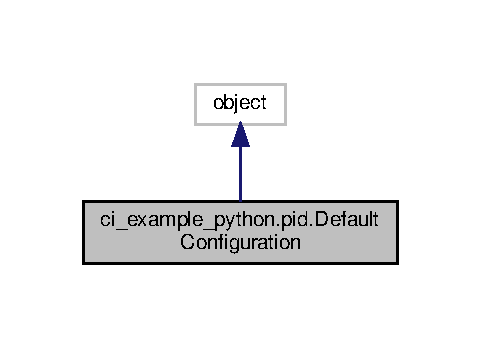
\includegraphics[width=231pt]{classci__example__python_1_1pid_1_1DefaultConfiguration__inherit__graph}
\end{center}
\end{figure}


Collaboration diagram for ci\+\_\+example\+\_\+python.\+pid.\+Default\+Configuration\+:
\nopagebreak
\begin{figure}[H]
\begin{center}
\leavevmode
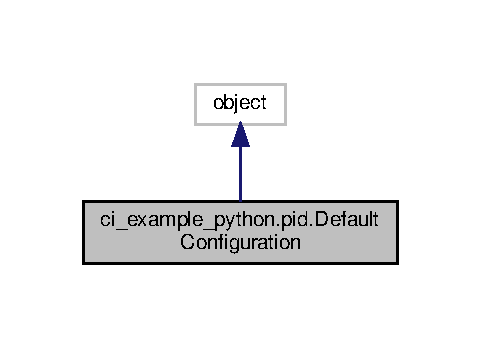
\includegraphics[width=231pt]{classci__example__python_1_1pid_1_1DefaultConfiguration__coll__graph}
\end{center}
\end{figure}
\subsection*{Static Public Attributes}
\begin{DoxyCompactItemize}
\item 
int \hyperlink{classci__example__python_1_1pid_1_1DefaultConfiguration_a8cda5972b7f42321a1100e636449edc0}{kp} = 1
\begin{DoxyCompactList}\small\item\em Proportional gain. \end{DoxyCompactList}\item 
int \hyperlink{classci__example__python_1_1pid_1_1DefaultConfiguration_a55077386d5f7c1fc5a24c6e0749b7678}{kd} = 1
\begin{DoxyCompactList}\small\item\em Derivative gain. \end{DoxyCompactList}\item 
int \hyperlink{classci__example__python_1_1pid_1_1DefaultConfiguration_ab390c7d434abe3ac47bff24d576f23d2}{ki} = 1
\begin{DoxyCompactList}\small\item\em Integral gain. \end{DoxyCompactList}\end{DoxyCompactItemize}


\subsection{Detailed Description}
\hyperlink{classci__example__python_1_1pid_1_1PID}{P\+ID} configuration. 

Configuration object with default values for kp, kd and ki can be used as input argument to create an instance of \hyperlink{classci__example__python_1_1pid_1_1PID}{P\+ID} \begin{DoxySeeAlso}{See also}
\hyperlink{classci__example__python_1_1pid_1_1PID}{P\+ID} 
\end{DoxySeeAlso}


\subsection{Member Data Documentation}
\mbox{\Hypertarget{classci__example__python_1_1pid_1_1DefaultConfiguration_a55077386d5f7c1fc5a24c6e0749b7678}\label{classci__example__python_1_1pid_1_1DefaultConfiguration_a55077386d5f7c1fc5a24c6e0749b7678}} 
\index{ci\+\_\+example\+\_\+python\+::pid\+::\+Default\+Configuration@{ci\+\_\+example\+\_\+python\+::pid\+::\+Default\+Configuration}!kd@{kd}}
\index{kd@{kd}!ci\+\_\+example\+\_\+python\+::pid\+::\+Default\+Configuration@{ci\+\_\+example\+\_\+python\+::pid\+::\+Default\+Configuration}}
\subsubsection{\texorpdfstring{kd}{kd}}
{\footnotesize\ttfamily ci\+\_\+example\+\_\+python.\+pid.\+Default\+Configuration.\+kd = 1\hspace{0.3cm}{\ttfamily [static]}}



Derivative gain. 

\mbox{\Hypertarget{classci__example__python_1_1pid_1_1DefaultConfiguration_ab390c7d434abe3ac47bff24d576f23d2}\label{classci__example__python_1_1pid_1_1DefaultConfiguration_ab390c7d434abe3ac47bff24d576f23d2}} 
\index{ci\+\_\+example\+\_\+python\+::pid\+::\+Default\+Configuration@{ci\+\_\+example\+\_\+python\+::pid\+::\+Default\+Configuration}!ki@{ki}}
\index{ki@{ki}!ci\+\_\+example\+\_\+python\+::pid\+::\+Default\+Configuration@{ci\+\_\+example\+\_\+python\+::pid\+::\+Default\+Configuration}}
\subsubsection{\texorpdfstring{ki}{ki}}
{\footnotesize\ttfamily ci\+\_\+example\+\_\+python.\+pid.\+Default\+Configuration.\+ki = 1\hspace{0.3cm}{\ttfamily [static]}}



Integral gain. 

\mbox{\Hypertarget{classci__example__python_1_1pid_1_1DefaultConfiguration_a8cda5972b7f42321a1100e636449edc0}\label{classci__example__python_1_1pid_1_1DefaultConfiguration_a8cda5972b7f42321a1100e636449edc0}} 
\index{ci\+\_\+example\+\_\+python\+::pid\+::\+Default\+Configuration@{ci\+\_\+example\+\_\+python\+::pid\+::\+Default\+Configuration}!kp@{kp}}
\index{kp@{kp}!ci\+\_\+example\+\_\+python\+::pid\+::\+Default\+Configuration@{ci\+\_\+example\+\_\+python\+::pid\+::\+Default\+Configuration}}
\subsubsection{\texorpdfstring{kp}{kp}}
{\footnotesize\ttfamily ci\+\_\+example\+\_\+python.\+pid.\+Default\+Configuration.\+kp = 1\hspace{0.3cm}{\ttfamily [static]}}



Proportional gain. 



The documentation for this class was generated from the following file\+:\begin{DoxyCompactItemize}
\item 
python/ci\+\_\+example\+\_\+python/\hyperlink{pid_8py}{pid.\+py}\end{DoxyCompactItemize}

\hypertarget{classci__example__python_1_1pid_1_1PID}{}\section{ci\+\_\+example\+\_\+python.\+pid.\+P\+ID Class Reference}
\label{classci__example__python_1_1pid_1_1PID}\index{ci\+\_\+example\+\_\+python.\+pid.\+P\+ID@{ci\+\_\+example\+\_\+python.\+pid.\+P\+ID}}


Simple 1D \hyperlink{classci__example__python_1_1pid_1_1PID}{P\+ID} controller.  


\subsection*{Public Member Functions}
\begin{DoxyCompactItemize}
\item 
def \hyperlink{classci__example__python_1_1pid_1_1PID_a904d0150a78efa3d5a3b7483aa310776}{\+\_\+\+\_\+init\+\_\+\+\_\+} (self, configuration)
\begin{DoxyCompactList}\small\item\em Constructor, initiallize the \hyperlink{classci__example__python_1_1pid_1_1PID}{P\+ID} gains from a given configuration. \end{DoxyCompactList}\item 
def \hyperlink{classci__example__python_1_1pid_1_1PID_a5810a7e3cf5db4ab2752e5d1502be766}{get\+\_\+gains} (self)
\begin{DoxyCompactList}\small\item\em Get the gains in a dictionary, keys\+: \char`\"{}kp\char`\"{}, \char`\"{}kd\char`\"{} and \char`\"{}ki\char`\"{}. \end{DoxyCompactList}\item 
\mbox{\Hypertarget{classci__example__python_1_1pid_1_1PID_a8958d8b988959214b187539939030baa}\label{classci__example__python_1_1pid_1_1PID_a8958d8b988959214b187539939030baa}} 
def \hyperlink{classci__example__python_1_1pid_1_1PID_a8958d8b988959214b187539939030baa}{reset\+\_\+integral} (self)
\begin{DoxyCompactList}\small\item\em Reset integral part of the \hyperlink{classci__example__python_1_1pid_1_1PID}{P\+ID} to 0.\+0. \end{DoxyCompactList}\item 
def \hyperlink{classci__example__python_1_1pid_1_1PID_aca3a513839029dd9cd7f46cff130c4ab}{compute} (self, position, velocity, position\+\_\+target, delta\+\_\+time)
\begin{DoxyCompactList}\small\item\em Compute the force related to the pid controller. \end{DoxyCompactList}\item 
\mbox{\Hypertarget{classci__example__python_1_1pid_1_1PID_a55e1d7ef174e9eb02566a5b674591da7}\label{classci__example__python_1_1pid_1_1PID_a55e1d7ef174e9eb02566a5b674591da7}} 
def \hyperlink{classci__example__python_1_1pid_1_1PID_a55e1d7ef174e9eb02566a5b674591da7}{\+\_\+\+\_\+str\+\_\+\+\_\+} (self)
\begin{DoxyCompactList}\small\item\em Convert the object into a string. \end{DoxyCompactList}\end{DoxyCompactItemize}
\subsection*{Private Attributes}
\begin{DoxyCompactItemize}
\item 
\hyperlink{classci__example__python_1_1pid_1_1PID_aee04c262f9b064702e13dd864f6b6f0f}{\+\_\+configuration}
\begin{DoxyCompactList}\small\item\em The \hyperlink{classci__example__python_1_1pid_1_1PID}{P\+ID} gains. \end{DoxyCompactList}\item 
\hyperlink{classci__example__python_1_1pid_1_1PID_a26b060dae844d341f5445980e869ba15}{\+\_\+integral}
\begin{DoxyCompactList}\small\item\em The integral term. \end{DoxyCompactList}\end{DoxyCompactItemize}


\subsection{Detailed Description}
Simple 1D \hyperlink{classci__example__python_1_1pid_1_1PID}{P\+ID} controller. 



\subsection{Constructor \& Destructor Documentation}
\mbox{\Hypertarget{classci__example__python_1_1pid_1_1PID_a904d0150a78efa3d5a3b7483aa310776}\label{classci__example__python_1_1pid_1_1PID_a904d0150a78efa3d5a3b7483aa310776}} 
\index{ci\+\_\+example\+\_\+python\+::pid\+::\+P\+ID@{ci\+\_\+example\+\_\+python\+::pid\+::\+P\+ID}!\+\_\+\+\_\+init\+\_\+\+\_\+@{\+\_\+\+\_\+init\+\_\+\+\_\+}}
\index{\+\_\+\+\_\+init\+\_\+\+\_\+@{\+\_\+\+\_\+init\+\_\+\+\_\+}!ci\+\_\+example\+\_\+python\+::pid\+::\+P\+ID@{ci\+\_\+example\+\_\+python\+::pid\+::\+P\+ID}}
\subsubsection{\texorpdfstring{\+\_\+\+\_\+init\+\_\+\+\_\+()}{\_\_init\_\_()}}
{\footnotesize\ttfamily def ci\+\_\+example\+\_\+python.\+pid.\+P\+I\+D.\+\_\+\+\_\+init\+\_\+\+\_\+ (\begin{DoxyParamCaption}\item[{}]{self,  }\item[{}]{configuration }\end{DoxyParamCaption})}



Constructor, initiallize the \hyperlink{classci__example__python_1_1pid_1_1PID}{P\+ID} gains from a given configuration. 


\begin{DoxyParams}{Parameters}
{\em configuration} & Any object with \char`\"{}kp\char`\"{}, \char`\"{}kd\char`\"{} and \char`\"{}ki\char`\"{} attributes (as float) \\
\hline
\end{DoxyParams}


\subsection{Member Function Documentation}
\mbox{\Hypertarget{classci__example__python_1_1pid_1_1PID_aca3a513839029dd9cd7f46cff130c4ab}\label{classci__example__python_1_1pid_1_1PID_aca3a513839029dd9cd7f46cff130c4ab}} 
\index{ci\+\_\+example\+\_\+python\+::pid\+::\+P\+ID@{ci\+\_\+example\+\_\+python\+::pid\+::\+P\+ID}!compute@{compute}}
\index{compute@{compute}!ci\+\_\+example\+\_\+python\+::pid\+::\+P\+ID@{ci\+\_\+example\+\_\+python\+::pid\+::\+P\+ID}}
\subsubsection{\texorpdfstring{compute()}{compute()}}
{\footnotesize\ttfamily def ci\+\_\+example\+\_\+python.\+pid.\+P\+I\+D.\+compute (\begin{DoxyParamCaption}\item[{}]{self,  }\item[{}]{position,  }\item[{}]{velocity,  }\item[{}]{position\+\_\+target,  }\item[{}]{delta\+\_\+time }\end{DoxyParamCaption})}



Compute the force related to the pid controller. 

This function is not stateless, as it performs integration. Call \hyperlink{classci__example__python_1_1pid_1_1PID_a8958d8b988959214b187539939030baa}{reset\+\_\+integral()} to reset the integral part.


\begin{DoxyParams}{Parameters}
{\em position} & Float {\ttfamily -\/-\/} current position \\
\hline
{\em velocity} & Float {\ttfamily -\/-\/} current velocity \\
\hline
{\em position\+\_\+target} & Float {\ttfamily -\/-\/} target position \\
\hline
{\em delta\+\_\+time} & Float {\ttfamily -\/-\/} time passed since last measurement. Used for integral computation \\
\hline
\end{DoxyParams}
\begin{DoxyReturn}{Returns}
Float {\ttfamily -\/-\/} computed force 
\end{DoxyReturn}
\mbox{\Hypertarget{classci__example__python_1_1pid_1_1PID_a5810a7e3cf5db4ab2752e5d1502be766}\label{classci__example__python_1_1pid_1_1PID_a5810a7e3cf5db4ab2752e5d1502be766}} 
\index{ci\+\_\+example\+\_\+python\+::pid\+::\+P\+ID@{ci\+\_\+example\+\_\+python\+::pid\+::\+P\+ID}!get\+\_\+gains@{get\+\_\+gains}}
\index{get\+\_\+gains@{get\+\_\+gains}!ci\+\_\+example\+\_\+python\+::pid\+::\+P\+ID@{ci\+\_\+example\+\_\+python\+::pid\+::\+P\+ID}}
\subsubsection{\texorpdfstring{get\+\_\+gains()}{get\_gains()}}
{\footnotesize\ttfamily def ci\+\_\+example\+\_\+python.\+pid.\+P\+I\+D.\+get\+\_\+gains (\begin{DoxyParamCaption}\item[{}]{self }\end{DoxyParamCaption})}



Get the gains in a dictionary, keys\+: \char`\"{}kp\char`\"{}, \char`\"{}kd\char`\"{} and \char`\"{}ki\char`\"{}. 

\begin{DoxyReturn}{Returns}
Dict {\ttfamily -\/-\/} The \hyperlink{classci__example__python_1_1pid_1_1PID}{P\+ID} gains. 
\end{DoxyReturn}


\subsection{Member Data Documentation}
\mbox{\Hypertarget{classci__example__python_1_1pid_1_1PID_aee04c262f9b064702e13dd864f6b6f0f}\label{classci__example__python_1_1pid_1_1PID_aee04c262f9b064702e13dd864f6b6f0f}} 
\index{ci\+\_\+example\+\_\+python\+::pid\+::\+P\+ID@{ci\+\_\+example\+\_\+python\+::pid\+::\+P\+ID}!\+\_\+configuration@{\+\_\+configuration}}
\index{\+\_\+configuration@{\+\_\+configuration}!ci\+\_\+example\+\_\+python\+::pid\+::\+P\+ID@{ci\+\_\+example\+\_\+python\+::pid\+::\+P\+ID}}
\subsubsection{\texorpdfstring{\+\_\+configuration}{\_configuration}}
{\footnotesize\ttfamily ci\+\_\+example\+\_\+python.\+pid.\+P\+I\+D.\+\_\+configuration\hspace{0.3cm}{\ttfamily [private]}}



The \hyperlink{classci__example__python_1_1pid_1_1PID}{P\+ID} gains. 

\mbox{\Hypertarget{classci__example__python_1_1pid_1_1PID_a26b060dae844d341f5445980e869ba15}\label{classci__example__python_1_1pid_1_1PID_a26b060dae844d341f5445980e869ba15}} 
\index{ci\+\_\+example\+\_\+python\+::pid\+::\+P\+ID@{ci\+\_\+example\+\_\+python\+::pid\+::\+P\+ID}!\+\_\+integral@{\+\_\+integral}}
\index{\+\_\+integral@{\+\_\+integral}!ci\+\_\+example\+\_\+python\+::pid\+::\+P\+ID@{ci\+\_\+example\+\_\+python\+::pid\+::\+P\+ID}}
\subsubsection{\texorpdfstring{\+\_\+integral}{\_integral}}
{\footnotesize\ttfamily ci\+\_\+example\+\_\+python.\+pid.\+P\+I\+D.\+\_\+integral\hspace{0.3cm}{\ttfamily [private]}}



The integral term. 



The documentation for this class was generated from the following file\+:\begin{DoxyCompactItemize}
\item 
python/ci\+\_\+example\+\_\+python/\hyperlink{pid_8py}{pid.\+py}\end{DoxyCompactItemize}

\hypertarget{classci__example__python_1_1pid_1_1RosConfiguration}{}\section{ci\+\_\+example\+\_\+python.\+pid.\+Ros\+Configuration Class Reference}
\label{classci__example__python_1_1pid_1_1RosConfiguration}\index{ci\+\_\+example\+\_\+python.\+pid.\+Ros\+Configuration@{ci\+\_\+example\+\_\+python.\+pid.\+Ros\+Configuration}}


R\+OS param configuration.  


\subsection*{Static Public Attributes}
\begin{DoxyCompactItemize}
\item 
string \hyperlink{classci__example__python_1_1pid_1_1RosConfiguration_a95d55922c360a7b8505c688e7c70de1d}{R\+O\+S\+P\+A\+R\+A\+M\+\_\+\+KP} = \char`\"{}kp\char`\"{}
\begin{DoxyCompactList}\small\item\em Key for reading kp gain. \end{DoxyCompactList}\item 
string \hyperlink{classci__example__python_1_1pid_1_1RosConfiguration_afe83e20beed21a38cf5138fbc4f45c35}{R\+O\+S\+P\+A\+R\+A\+M\+\_\+\+KD} = \char`\"{}kd\char`\"{}
\begin{DoxyCompactList}\small\item\em Key for reading kd gain. \end{DoxyCompactList}\item 
string \hyperlink{classci__example__python_1_1pid_1_1RosConfiguration_af9a9bff01a2434fa29788b178e0a3afe}{R\+O\+S\+P\+A\+R\+A\+M\+\_\+\+KI} = \char`\"{}ki\char`\"{}
\begin{DoxyCompactList}\small\item\em Key for reading ki gain. \end{DoxyCompactList}\end{DoxyCompactItemize}


\subsection{Detailed Description}
R\+OS param configuration. 

This contains the name of the ros parameter server keys for the \hyperlink{classci__example__python_1_1pid_1_1PID}{P\+ID} gains. 

\subsection{Member Data Documentation}
\mbox{\Hypertarget{classci__example__python_1_1pid_1_1RosConfiguration_afe83e20beed21a38cf5138fbc4f45c35}\label{classci__example__python_1_1pid_1_1RosConfiguration_afe83e20beed21a38cf5138fbc4f45c35}} 
\index{ci\+\_\+example\+\_\+python\+::pid\+::\+Ros\+Configuration@{ci\+\_\+example\+\_\+python\+::pid\+::\+Ros\+Configuration}!R\+O\+S\+P\+A\+R\+A\+M\+\_\+\+KD@{R\+O\+S\+P\+A\+R\+A\+M\+\_\+\+KD}}
\index{R\+O\+S\+P\+A\+R\+A\+M\+\_\+\+KD@{R\+O\+S\+P\+A\+R\+A\+M\+\_\+\+KD}!ci\+\_\+example\+\_\+python\+::pid\+::\+Ros\+Configuration@{ci\+\_\+example\+\_\+python\+::pid\+::\+Ros\+Configuration}}
\subsubsection{\texorpdfstring{R\+O\+S\+P\+A\+R\+A\+M\+\_\+\+KD}{ROSPARAM\_KD}}
{\footnotesize\ttfamily ci\+\_\+example\+\_\+python.\+pid.\+Ros\+Configuration.\+R\+O\+S\+P\+A\+R\+A\+M\+\_\+\+KD = \char`\"{}kd\char`\"{}\hspace{0.3cm}{\ttfamily [static]}}



Key for reading kd gain. 

\mbox{\Hypertarget{classci__example__python_1_1pid_1_1RosConfiguration_af9a9bff01a2434fa29788b178e0a3afe}\label{classci__example__python_1_1pid_1_1RosConfiguration_af9a9bff01a2434fa29788b178e0a3afe}} 
\index{ci\+\_\+example\+\_\+python\+::pid\+::\+Ros\+Configuration@{ci\+\_\+example\+\_\+python\+::pid\+::\+Ros\+Configuration}!R\+O\+S\+P\+A\+R\+A\+M\+\_\+\+KI@{R\+O\+S\+P\+A\+R\+A\+M\+\_\+\+KI}}
\index{R\+O\+S\+P\+A\+R\+A\+M\+\_\+\+KI@{R\+O\+S\+P\+A\+R\+A\+M\+\_\+\+KI}!ci\+\_\+example\+\_\+python\+::pid\+::\+Ros\+Configuration@{ci\+\_\+example\+\_\+python\+::pid\+::\+Ros\+Configuration}}
\subsubsection{\texorpdfstring{R\+O\+S\+P\+A\+R\+A\+M\+\_\+\+KI}{ROSPARAM\_KI}}
{\footnotesize\ttfamily ci\+\_\+example\+\_\+python.\+pid.\+Ros\+Configuration.\+R\+O\+S\+P\+A\+R\+A\+M\+\_\+\+KI = \char`\"{}ki\char`\"{}\hspace{0.3cm}{\ttfamily [static]}}



Key for reading ki gain. 

\mbox{\Hypertarget{classci__example__python_1_1pid_1_1RosConfiguration_a95d55922c360a7b8505c688e7c70de1d}\label{classci__example__python_1_1pid_1_1RosConfiguration_a95d55922c360a7b8505c688e7c70de1d}} 
\index{ci\+\_\+example\+\_\+python\+::pid\+::\+Ros\+Configuration@{ci\+\_\+example\+\_\+python\+::pid\+::\+Ros\+Configuration}!R\+O\+S\+P\+A\+R\+A\+M\+\_\+\+KP@{R\+O\+S\+P\+A\+R\+A\+M\+\_\+\+KP}}
\index{R\+O\+S\+P\+A\+R\+A\+M\+\_\+\+KP@{R\+O\+S\+P\+A\+R\+A\+M\+\_\+\+KP}!ci\+\_\+example\+\_\+python\+::pid\+::\+Ros\+Configuration@{ci\+\_\+example\+\_\+python\+::pid\+::\+Ros\+Configuration}}
\subsubsection{\texorpdfstring{R\+O\+S\+P\+A\+R\+A\+M\+\_\+\+KP}{ROSPARAM\_KP}}
{\footnotesize\ttfamily ci\+\_\+example\+\_\+python.\+pid.\+Ros\+Configuration.\+R\+O\+S\+P\+A\+R\+A\+M\+\_\+\+KP = \char`\"{}kp\char`\"{}\hspace{0.3cm}{\ttfamily [static]}}



Key for reading kp gain. 



The documentation for this class was generated from the following file\+:\begin{DoxyCompactItemize}
\item 
python/ci\+\_\+example\+\_\+python/\hyperlink{pid_8py}{pid.\+py}\end{DoxyCompactItemize}

\chapter{File Documentation}
\hypertarget{demo__pid_8py}{}\section{demos/demo\+\_\+pid.py File Reference}
\label{demo__pid_8py}\index{demos/demo\+\_\+pid.\+py@{demos/demo\+\_\+pid.\+py}}
\subsection*{Classes}
\begin{DoxyCompactItemize}
\item 
class \hyperlink{classdemo__pid_1_1Configuration}{demo\+\_\+pid.\+Configuration}
\begin{DoxyCompactList}\small\item\em This a small shell that contains the P\+ID gains. \end{DoxyCompactList}\end{DoxyCompactItemize}
\subsection*{Namespaces}
\begin{DoxyCompactItemize}
\item 
 \hyperlink{namespaceDemos}{Demos}
\begin{DoxyCompactList}\small\item\em of the \hyperlink{classci__example__python_1_1pid_1_1PID}{ci\+\_\+example\+\_\+python.\+pid.\+P\+ID} controller. \end{DoxyCompactList}\end{DoxyCompactItemize}
\subsection*{Variables}
\begin{DoxyCompactItemize}
\item 
\mbox{\Hypertarget{demo__pid_8py_a7b7423815d4198f332e68658b6c596cc}\label{demo__pid_8py_a7b7423815d4198f332e68658b6c596cc}} 
int \hyperlink{demo__pid_8py_a7b7423815d4198f332e68658b6c596cc}{demo\+\_\+pid.\+current\+\_\+position} = 1
\begin{DoxyCompactList}\small\item\em Input position for the pid controller. \end{DoxyCompactList}\item 
\mbox{\Hypertarget{demo__pid_8py_a871d2c19b8b54eb80984deea3be9dd27}\label{demo__pid_8py_a871d2c19b8b54eb80984deea3be9dd27}} 
float \hyperlink{demo__pid_8py_a871d2c19b8b54eb80984deea3be9dd27}{demo\+\_\+pid.\+current\+\_\+velocity} = 0.\+1
\begin{DoxyCompactList}\small\item\em Input velcoity for the pid controller. \end{DoxyCompactList}\item 
\mbox{\Hypertarget{demo__pid_8py_af83ebb1dca4291be9f3b51161b6b840a}\label{demo__pid_8py_af83ebb1dca4291be9f3b51161b6b840a}} 
int \hyperlink{demo__pid_8py_af83ebb1dca4291be9f3b51161b6b840a}{demo\+\_\+pid.\+position\+\_\+target} = 0
\begin{DoxyCompactList}\small\item\em Input target position for the pid controller. \end{DoxyCompactList}\item 
\mbox{\Hypertarget{demo__pid_8py_aff195a0d0ed388ecbac82279f72e8453}\label{demo__pid_8py_aff195a0d0ed388ecbac82279f72e8453}} 
float \hyperlink{demo__pid_8py_aff195a0d0ed388ecbac82279f72e8453}{demo\+\_\+pid.\+delta\+\_\+time} = 0.\+001
\begin{DoxyCompactList}\small\item\em Input smapling period for the pid controller. \end{DoxyCompactList}\item 
\mbox{\Hypertarget{demo__pid_8py_af6615cc84ca31e150aad2c07af78f190}\label{demo__pid_8py_af6615cc84ca31e150aad2c07af78f190}} 
\hyperlink{demo__pid_8py_af6615cc84ca31e150aad2c07af78f190}{demo\+\_\+pid.\+config} = Configuration(1,1,1)
\begin{DoxyCompactList}\small\item\em \hyperlink{classdemo__pid_1_1Configuration}{Configuration} of the P\+ID controller. \end{DoxyCompactList}\item 
\hyperlink{demo__pid_8py_aad8a5d0c0daf5c450a03fb9c5043c11f}{demo\+\_\+pid.\+pid} = P\+ID(config)
\begin{DoxyCompactList}\small\item\em Example of creation of the P\+ID using a config class. \end{DoxyCompactList}\item 
\hyperlink{demo__pid_8py_abb2c07c72cb1d855cf8026a44b006468}{demo\+\_\+pid.\+force} = pid.\+compute(current\+\_\+position,current\+\_\+velocity,position\+\_\+target,delta\+\_\+time)
\begin{DoxyCompactList}\small\item\em Compute the control from the current input. \end{DoxyCompactList}\end{DoxyCompactItemize}


\subsection{Detailed Description}
\begin{DoxyCopyright}{Copyright}
Copyright (c) 2017-\/2019, New York University and Max Planck Gesellschaft, License B\+S\+D-\/3-\/\+Clause 
\end{DoxyCopyright}


\subsection{Variable Documentation}
\mbox{\Hypertarget{demo__pid_8py_file_abb2c07c72cb1d855cf8026a44b006468}\label{demo__pid_8py_file_abb2c07c72cb1d855cf8026a44b006468}} 
\index{demo\+\_\+pid.\+py@{demo\+\_\+pid.\+py}!force@{force}}
\index{force@{force}!demo\+\_\+pid.\+py@{demo\+\_\+pid.\+py}}
\subsubsection{\texorpdfstring{force}{force}}
{\footnotesize\ttfamily demo\+\_\+pid.\+force = pid.\+compute(current\+\_\+position,current\+\_\+velocity,position\+\_\+target,delta\+\_\+time)}



Compute the control from the current input. 

\mbox{\Hypertarget{demo__pid_8py_file_aad8a5d0c0daf5c450a03fb9c5043c11f}\label{demo__pid_8py_file_aad8a5d0c0daf5c450a03fb9c5043c11f}} 
\index{demo\+\_\+pid.\+py@{demo\+\_\+pid.\+py}!pid@{pid}}
\index{pid@{pid}!demo\+\_\+pid.\+py@{demo\+\_\+pid.\+py}}
\subsubsection{\texorpdfstring{pid}{pid}}
{\footnotesize\ttfamily demo\+\_\+pid.\+pid = P\+ID(config)}



Example of creation of the P\+ID using a config class. 

Example of creation of the P\+ID using default gains.
\hypertarget{demo__ros__pid_8py}{}\section{demos/demo\+\_\+ros\+\_\+pid.py File Reference}
\label{demo__ros__pid_8py}\index{demos/demo\+\_\+ros\+\_\+pid.\+py@{demos/demo\+\_\+ros\+\_\+pid.\+py}}
\subsection*{Namespaces}
\begin{DoxyCompactItemize}
\item 
 \hyperlink{namespaceDemos}{Demos}
\begin{DoxyCompactList}\small\item\em of the \hyperlink{classci__example__python_1_1pid_1_1PID}{ci\+\_\+example\+\_\+python.\+pid.\+P\+ID} controller. \end{DoxyCompactList}\end{DoxyCompactItemize}
\subsection*{Variables}
\begin{DoxyCompactItemize}
\item 
\mbox{\Hypertarget{demo__ros__pid_8py_a08225519cc11ebf24c572a0430b1605f}\label{demo__ros__pid_8py_a08225519cc11ebf24c572a0430b1605f}} 
int \hyperlink{demo__ros__pid_8py_a08225519cc11ebf24c572a0430b1605f}{demo\+\_\+ros\+\_\+pid.\+current\+\_\+position} = 1
\begin{DoxyCompactList}\small\item\em Input position for the pid controller. \end{DoxyCompactList}\item 
\mbox{\Hypertarget{demo__ros__pid_8py_a87dfecd3418484a7047c40e07add0673}\label{demo__ros__pid_8py_a87dfecd3418484a7047c40e07add0673}} 
float \hyperlink{demo__ros__pid_8py_a87dfecd3418484a7047c40e07add0673}{demo\+\_\+ros\+\_\+pid.\+current\+\_\+velocity} = 0.\+1
\begin{DoxyCompactList}\small\item\em Input velcoity for the pid controller. \end{DoxyCompactList}\item 
\mbox{\Hypertarget{demo__ros__pid_8py_a753feefb93ca5750e9a00d68b3695cb6}\label{demo__ros__pid_8py_a753feefb93ca5750e9a00d68b3695cb6}} 
int \hyperlink{demo__ros__pid_8py_a753feefb93ca5750e9a00d68b3695cb6}{demo\+\_\+ros\+\_\+pid.\+position\+\_\+target} = 0
\begin{DoxyCompactList}\small\item\em Input target position for the pid controller. \end{DoxyCompactList}\item 
\mbox{\Hypertarget{demo__ros__pid_8py_a61446e4f52ef5778ea45e665f806d091}\label{demo__ros__pid_8py_a61446e4f52ef5778ea45e665f806d091}} 
float \hyperlink{demo__ros__pid_8py_a61446e4f52ef5778ea45e665f806d091}{demo\+\_\+ros\+\_\+pid.\+delta\+\_\+time} = 0.\+001
\begin{DoxyCompactList}\small\item\em Input smapling period for the pid controller. \end{DoxyCompactList}\item 
\hyperlink{demo__ros__pid_8py_a791119bb7d8fb5604109583788b6cc37}{demo\+\_\+ros\+\_\+pid.\+pid} = get\+\_\+ros\+\_\+params\+\_\+pid()
\begin{DoxyCompactList}\small\item\em Example of creation of P\+ID using default gains. \end{DoxyCompactList}\item 
\hyperlink{demo__ros__pid_8py_aee57a126e7df8e246d9fa37a3bfdb58b}{demo\+\_\+ros\+\_\+pid.\+control} = pid.\+compute(current\+\_\+position,current\+\_\+velocity,position\+\_\+target,delta\+\_\+time)
\begin{DoxyCompactList}\small\item\em Compute the control from the current input. \end{DoxyCompactList}\end{DoxyCompactItemize}


\subsection{Detailed Description}
\begin{DoxyCopyright}{Copyright}
Copyright (c) 2017-\/2019, New York University and Max Planck Gesellschaft, License B\+S\+D-\/3-\/\+Clause 
\end{DoxyCopyright}


\subsection{Variable Documentation}
\mbox{\Hypertarget{demo__ros__pid_8py_file_aee57a126e7df8e246d9fa37a3bfdb58b}\label{demo__ros__pid_8py_file_aee57a126e7df8e246d9fa37a3bfdb58b}} 
\index{demo\+\_\+ros\+\_\+pid.\+py@{demo\+\_\+ros\+\_\+pid.\+py}!control@{control}}
\index{control@{control}!demo\+\_\+ros\+\_\+pid.\+py@{demo\+\_\+ros\+\_\+pid.\+py}}
\subsubsection{\texorpdfstring{control}{control}}
{\footnotesize\ttfamily demo\+\_\+ros\+\_\+pid.\+control = pid.\+compute(current\+\_\+position,current\+\_\+velocity,position\+\_\+target,delta\+\_\+time)}



Compute the control from the current input. 

\mbox{\Hypertarget{demo__ros__pid_8py_file_a791119bb7d8fb5604109583788b6cc37}\label{demo__ros__pid_8py_file_a791119bb7d8fb5604109583788b6cc37}} 
\index{demo\+\_\+ros\+\_\+pid.\+py@{demo\+\_\+ros\+\_\+pid.\+py}!pid@{pid}}
\index{pid@{pid}!demo\+\_\+ros\+\_\+pid.\+py@{demo\+\_\+ros\+\_\+pid.\+py}}
\subsubsection{\texorpdfstring{pid}{pid}}
{\footnotesize\ttfamily demo\+\_\+ros\+\_\+pid.\+pid = get\+\_\+ros\+\_\+params\+\_\+pid()}



Example of creation of P\+ID using default gains. 


\hypertarget{____init_____8py}{}\section{python/mpi\+\_\+cmake\+\_\+modules/\+\_\+\+\_\+init\+\_\+\+\_\+.py File Reference}
\label{____init_____8py}\index{python/mpi\+\_\+cmake\+\_\+modules/\+\_\+\+\_\+init\+\_\+\+\_\+.\+py@{python/mpi\+\_\+cmake\+\_\+modules/\+\_\+\+\_\+init\+\_\+\+\_\+.\+py}}


\subsection{Detailed Description}
\begin{DoxyRefDesc}{License}
\item[\hyperlink{license__license000001}{License}]License B\+S\+D-\/3-\/\+Clause \end{DoxyRefDesc}
\begin{DoxyCopyright}{Copyright}
Copyright (c) 2019, New York University and Max Planck Gesellschaft. 
\end{DoxyCopyright}

\hypertarget{pid_8py}{}\section{python/ci\+\_\+example\+\_\+python/pid.py File Reference}
\label{pid_8py}\index{python/ci\+\_\+example\+\_\+python/pid.\+py@{python/ci\+\_\+example\+\_\+python/pid.\+py}}
\subsection*{Classes}
\begin{DoxyCompactItemize}
\item 
class \hyperlink{classci__example__python_1_1pid_1_1DefaultConfiguration}{ci\+\_\+example\+\_\+python.\+pid.\+Default\+Configuration}
\begin{DoxyCompactList}\small\item\em \hyperlink{classci__example__python_1_1pid_1_1PID}{P\+ID} configuration. \end{DoxyCompactList}\item 
class \hyperlink{classci__example__python_1_1pid_1_1RosConfiguration}{ci\+\_\+example\+\_\+python.\+pid.\+Ros\+Configuration}
\begin{DoxyCompactList}\small\item\em R\+OS param configuration. \end{DoxyCompactList}\item 
class \hyperlink{classci__example__python_1_1pid_1_1ConfigFileConfiguration}{ci\+\_\+example\+\_\+python.\+pid.\+Config\+File\+Configuration}
\begin{DoxyCompactList}\small\item\em Path to default configuration file, relative to the pid package. \end{DoxyCompactList}\item 
class \hyperlink{classci__example__python_1_1pid_1_1PID}{ci\+\_\+example\+\_\+python.\+pid.\+P\+ID}
\begin{DoxyCompactList}\small\item\em Simple 1D \hyperlink{classci__example__python_1_1pid_1_1PID}{P\+ID} controller. \end{DoxyCompactList}\end{DoxyCompactItemize}
\subsection*{Namespaces}
\begin{DoxyCompactItemize}
\item 
 \hyperlink{namespaceci__example__python_1_1pid}{ci\+\_\+example\+\_\+python.\+pid}
\begin{DoxyCompactList}\small\item\em Brief description of the pid module. \end{DoxyCompactList}\end{DoxyCompactItemize}
\subsection*{Functions}
\begin{DoxyCompactItemize}
\item 
def \hyperlink{namespaceci__example__python_1_1pid_ae3cae0234e7c25f408cddd004494c5ca}{ci\+\_\+example\+\_\+python.\+pid.\+\_\+read\+\_\+yaml\+\_\+config\+\_\+file} (file\+\_\+path)
\begin{DoxyCompactList}\small\item\em Parse a yaml file to get the \hyperlink{classci__example__python_1_1pid_1_1PID}{P\+ID} gains. \end{DoxyCompactList}\item 
def \hyperlink{namespaceci__example__python_1_1pid_a6fc811a84ce986b8315aabae71987cbf}{ci\+\_\+example\+\_\+python.\+pid.\+get\+\_\+default\+\_\+pid} ()
\begin{DoxyCompactList}\small\item\em Factory for default \hyperlink{classci__example__python_1_1pid_1_1PID}{P\+ID} controller. \end{DoxyCompactList}\item 
def \hyperlink{namespaceci__example__python_1_1pid_ae1f8a5e73e269ede0bdd4d0daf2f265e}{ci\+\_\+example\+\_\+python.\+pid.\+get\+\_\+ros\+\_\+params\+\_\+pid} (verbose=True)
\begin{DoxyCompactList}\small\item\em Get a \hyperlink{classci__example__python_1_1pid_1_1PID}{P\+ID} controller paramterized through R\+OS params. \end{DoxyCompactList}\item 
def \hyperlink{namespaceci__example__python_1_1pid_a18376955fadc78cf60e9836c120adc9a}{ci\+\_\+example\+\_\+python.\+pid.\+get\+\_\+config\+\_\+file\+\_\+pid} (config\+\_\+file\+\_\+path=None, verbose=True)
\begin{DoxyCompactList}\small\item\em Reads a yaml file and return a corresponding \hyperlink{classci__example__python_1_1pid_1_1PID}{P\+ID} controller. \end{DoxyCompactList}\end{DoxyCompactItemize}


\subsection{Detailed Description}
\begin{DoxyCopyright}{Copyright}
Copyright (c) 2017-\/2019, New York University and Max Planck Gesellschaft, License B\+S\+D-\/3-\/\+Clause 
\end{DoxyCopyright}

\chapter{Example Documentation}
\hypertarget{demo_pid_8py-example}{}\section{demo\+\_\+pid.\+py}
In order to run this demos the {\ttfamily ci\+\_\+example\+\_\+python/python/ci\+\_\+example\+\_\+python} path needs to be added in the {\ttfamily P\+Y\+T\+H\+O\+N\+P\+A\+TH}. This is done after\+:
\begin{DoxyItemize}
\item 1. Building the workspace by executing {\ttfamily catkin\+\_\+make} from the root of the catkin workspace.
\item 2. \char`\"{}source ./devel/setup.\+bash\char`\"{} is called from the root of the catkin workspace.
\item 3. Run the demo by either\+:
\begin{DoxyItemize}
\item 3.\+1. {\ttfamily rosrun \hyperlink{namespaceci__example__python}{ci\+\_\+example\+\_\+python} \hyperlink{demo__pid_8py}{demo\+\_\+pid.\+py}}
\item 3.\+3. {\ttfamily cd /path/to/ci\+\_\+example\+\_\+python/} ; {\ttfamily ./demos/demo\+\_\+pid.py}
\end{DoxyItemize}
\end{DoxyItemize}

Notice the use of the double \#\# for the comments. This allow Doxygen to parse you code and for you to explain in details the content of the demo.


\begin{DoxyCodeInclude}
1 \textcolor{comment}{#!/usr/bin/env python}
2 
3 \textcolor{stringliteral}{""" @namespace Demos of the ci\_example\_python.pid.PID controller.}
4 \textcolor{stringliteral}{}
5 \textcolor{stringliteral}{@file demo\_pid.py}
6 \textcolor{stringliteral}{@copyright Copyright (c) 2017-2019,}
7 \textcolor{stringliteral}{           New York University and Max Planck Gesellschaft,}
8 \textcolor{stringliteral}{           License BSD-3-Clause}
9 \textcolor{stringliteral}{}
10 \textcolor{stringliteral}{@example demo\_pid.py}
11 \textcolor{stringliteral}{In order to run this demos the `ci\_example\_python/python/ci\_example\_python` path}
12 \textcolor{stringliteral}{needs to be added in the `PYTHONPATH`. This is done after:}
13 \textcolor{stringliteral}{- 1. Building the workspace by executing `catkin\_make` from the root of the}
14 \textcolor{stringliteral}{     catkin workspace.}
15 \textcolor{stringliteral}{- 2. "source ./devel/setup.bash" is called from the root of the catkin}
16 \textcolor{stringliteral}{     workspace.}
17 \textcolor{stringliteral}{- 3. Run the demo by either:}
18 \textcolor{stringliteral}{    - 3.1. `rosrun ci\_example\_python demo\_pid.py`}
19 \textcolor{stringliteral}{    - 3.3. `cd /path/to/ci\_example\_python/` ; `./demos/demo\_pid.py`}
20 \textcolor{stringliteral}{}
21 \textcolor{stringliteral}{Notice the use of the double ## for the comments. This allow Doxygen}
22 \textcolor{stringliteral}{to parse you code and for you to explain in details the content of the demo.}
23 \textcolor{stringliteral}{"""}
24 
25 
26 \textcolor{comment}{# Python 3 compatibility, has to be called just after the hashbang.}
27 \textcolor{keyword}{from} \_\_future\_\_ \textcolor{keyword}{import} print\_function, division
28 \textcolor{keyword}{from} \hyperlink{namespaceci__example__python_1_1pid}{ci\_example\_python.pid} \textcolor{keyword}{import} PID, get\_default\_pid, get\_config\_file\_pid
29 
30 
31 \textcolor{keywordflow}{if} \_\_name\_\_ == \textcolor{stringliteral}{"\_\_main\_\_"}:
32     
33     
34     current\_position = 1
35     
36     current\_velocity = 0.1
37     
38     position\_target = 0
39     
40     delta\_time = 0.001
41 
42     \textcolor{comment}{# basic example of PID usage}
43     print(\textcolor{stringliteral}{"basic pid usage:"})
44     
45     \textcolor{keyword}{class }Configuration:
46         \textcolor{stringliteral}{""" This a small shell that contains the PID gains.}
47 \textcolor{stringliteral}{        It mocks the load of a yaml files.}
48 \textcolor{stringliteral}{        Attributes:}
49 \textcolor{stringliteral}{            kp: Proportional gain.}
50 \textcolor{stringliteral}{            kd: Derivative gain.}
51 \textcolor{stringliteral}{            ki: Integral gain.}
52 \textcolor{stringliteral}{        """}
53         
54         \textcolor{keyword}{def }\_\_init\_\_(self, kp, kd, ki):
55             \textcolor{stringliteral}{"""  Create the 3 gains}
56 \textcolor{stringliteral}{            Args:}
57 \textcolor{stringliteral}{                kp: Proportional gain.}
58 \textcolor{stringliteral}{                kd: Derivative gain.}
59 \textcolor{stringliteral}{                ki: Integral gain.}
60 \textcolor{stringliteral}{            """}
61             self.kp = kp
62             self.kd = kd
63             self.ki = ki
64 
65     
66     config = Configuration(1,1,1)
67 
68     
69     pid = PID(config)
70     print(pid)
71     
72     force = pid.compute(current\_position,current\_velocity,position\_target,delta\_time)
73     print(\textcolor{stringliteral}{"force:"},force)
74 
75     
76     \textcolor{keywordflow}{print} (\textcolor{stringliteral}{"pid using default gains:"})
77     pid = \hyperlink{namespaceci__example__python_1_1pid_a6fc811a84ce986b8315aabae71987cbf}{get\_default\_pid}()
78     \textcolor{keywordflow}{print} (pid)
79 
80     force = pid.compute(current\_position,current\_velocity,position\_target,delta\_time)
81     \textcolor{keywordflow}{print} (\textcolor{stringliteral}{"force:"},force)
82 
83     \textcolor{comment}{# Example of creation of the PID using config files read from config file.}
84     \textcolor{keywordflow}{print} (\textcolor{stringliteral}{"pid using gains read from config file:"})
85     pid = \hyperlink{namespaceci__example__python_1_1pid_a18376955fadc78cf60e9836c120adc9a}{get\_config\_file\_pid}(verbose=\textcolor{keyword}{True})
86     \textcolor{keywordflow}{print} (pid)
87 
88     force = pid.compute(current\_position,current\_velocity,position\_target,delta\_time)
89     \textcolor{keywordflow}{print} (\textcolor{stringliteral}{"force:"},force)
\end{DoxyCodeInclude}
 
\hypertarget{demo_ros_pid_8py-example}{}\section{demo\+\_\+ros\+\_\+pid.\+py}
In order to run this demos the {\ttfamily ci\+\_\+example\+\_\+python/python/ci\+\_\+example\+\_\+python} path needs to be added in the {\ttfamily P\+Y\+T\+H\+O\+N\+P\+A\+TH}. This is done after\+:
\begin{DoxyItemize}
\item 1. \char`\"{}catkin\+\_\+make\char`\"{} is called from the root of the catkin workspace
\item 2. \char`\"{}source ./devel/setup.\+bash\char`\"{} is called from the root of the catkin workspace
\item 3. roscore is called in an additional terminal
\item 4. Finally run {\ttfamily rosrun \hyperlink{namespaceci__example__python}{ci\+\_\+example\+\_\+python} \hyperlink{demo__ros__pid_8py}{demo\+\_\+ros\+\_\+pid.\+py}}
\end{DoxyItemize}

Notice the use of the double \#\# for the comments. This allow Doxygen to parse you code and for you to explain in details the content of the demo.


\begin{DoxyCodeInclude}
1 \textcolor{comment}{#!/usr/bin/env python}
2 
3 
4 \textcolor{stringliteral}{""" @namespace Demos of the ci\_example\_python.pid.PID controller using ROS param.}
5 \textcolor{stringliteral}{}
6 \textcolor{stringliteral}{@file demo\_ros\_pid.py}
7 \textcolor{stringliteral}{@copyright Copyright (c) 2017-2019,}
8 \textcolor{stringliteral}{           New York University and Max Planck Gesellschaft,}
9 \textcolor{stringliteral}{           License BSD-3-Clause}
10 \textcolor{stringliteral}{}
11 \textcolor{stringliteral}{@example demo\_ros\_pid.py}
12 \textcolor{stringliteral}{In order to run this demos the `ci\_example\_python/python/ci\_example\_python` path}
13 \textcolor{stringliteral}{needs to be added in the `PYTHONPATH`. This is done after:}
14 \textcolor{stringliteral}{- 1. "catkin\_make" is called from the root of the catkin workspace}
15 \textcolor{stringliteral}{- 2. "source ./devel/setup.bash" is called from the root of the catkin workspace}
16 \textcolor{stringliteral}{- 3. roscore is called in an additional terminal}
17 \textcolor{stringliteral}{- 4. Finally run `rosrun ci\_example\_python demo\_ros\_pid.py`}
18 \textcolor{stringliteral}{}
19 \textcolor{stringliteral}{Notice the use of the double ## for the comments. This allow Doxygen}
20 \textcolor{stringliteral}{to parse you code and for you to explain in details the content of the demo.}
21 \textcolor{stringliteral}{"""}
22 
23 
24 \textcolor{comment}{# Python 3 compatibility, has to be called just after the hashbang.}
25 \textcolor{keyword}{from} \_\_future\_\_ \textcolor{keyword}{import} print\_function, division
26 \textcolor{keyword}{import} rospy
27 \textcolor{keyword}{from} \hyperlink{namespaceci__example__python_1_1pid}{ci\_example\_python.pid} \textcolor{keyword}{import} get\_ros\_params\_pid
28 
29 
30 \textcolor{keywordflow}{if} \_\_name\_\_ == \textcolor{stringliteral}{"\_\_main\_\_"}:
31     
32     \textcolor{comment}{# here we set the parameters to ROS.}
33     rospy.set\_param(\textcolor{stringliteral}{'kp'}, 1.0)
34     rospy.set\_param(\textcolor{stringliteral}{'kd'}, 1.0)
35     rospy.set\_param(\textcolor{stringliteral}{'ki'}, 1.0)
36 
37     
38     current\_position = 1
39     
40     current\_velocity = 0.1
41     
42     position\_target = 0
43     
44     delta\_time = 0.001
45 
46     \textcolor{keywordflow}{print} (\textcolor{stringliteral}{"pid using ros parameter server"})
47 
48     
49     pid = \hyperlink{namespaceci__example__python_1_1pid_ae1f8a5e73e269ede0bdd4d0daf2f265e}{get\_ros\_params\_pid}()
50     \textcolor{keywordflow}{print} (pid)
51 
52     
53     control = pid.compute(current\_position,current\_velocity,position\_target,delta\_time)
54     \textcolor{keywordflow}{print} (\textcolor{stringliteral}{"control: "},control)
\end{DoxyCodeInclude}
 
%--- End generated contents ---

% Index
\backmatter
\newpage
\phantomsection
\clearemptydoublepage
\addcontentsline{toc}{chapter}{Index}
\printindex

\end{document}
